%!TEX encoding = UTF-8 Unicode

% From OUP/Overleaf for Genetics, heavily modified by Nilo Merino Recalde:
% https://github.com/nilomr

\documentclass[9pt, twocolumn, twoside]{nilosthesis}
% set font to 9pt

% Use the documentclass option 'lineno' to view line numbers, and twocolumn to have two columns obviously
\usepackage{epstopdf}
\usepackage{orcidlink}
\usepackage{caption}
\usepackage{tipa}
\usepackage{doi}
\usepackage{tabularray}
\usepackage{tcolorbox}
\usepackage{hyperref}
\usepackage{multicol} % for multiple column layouts in the same document
\usepackage{setspace}
\setstretch{1.15} % body line space

\usetikzlibrary{external} % externalise tikz figures
\tikzexternalize


\begin{document}


% cover, frontispiece, etc ==============================

\bgroup
\hypersetup{linkcolor = black}
% add 3cm before the start
\tableofcontents

%\authorlist

\listoffigures
%\listoftables % there's just two tables really, so I don't think it's worth it
\egroup

% Chapter 1: Introduction ==============================


\runningauthor{Merino Recalde, 2023 }
\fancyhead[LE]{\sffamily\color{black50}\thepage\hspace{2em}General introduction}
%\runningtitle{General introduction}
\clearpage{\pagestyle{empty}\cleardoublepage} % empty page before chapter
\onecolumn % start one-column layout for chatper 4

    \chapter{Introduction}
    \vspace{10pt}
    \thispagestyle{empty}  % remove page number 

    \begin{chapquote}{Werner Herzog, \textit{Burden of Dreams (1982)}}
        [T]he birds are in misery. I don't think they---they sing, they just screech in pain. 
    \end{chapquote}
    
    \vspace{1cm}

% Begin chapter proper
\begin{multicols}{2} % start one-column layout
    \section{Animal culture and social learning }
The idea that culture demarcated humans from other animals used to be widespread in Western academia. Over the past few decades this view was steadily challenged, and today it is common to find references to non-human animal cultures in scientific journals and the popular press alike (Whiten 2019a). To be sure, some energetically oppose the notion, and there is no shortage of disagreement over the definition of the term ‘culture’ (Laland \& Hoppitt 2003; Heyes 2020; kroeber defs of cult). But intricate and distinctive as human culture might be, the now burgeoning field of animal cultural research is showing us that the difference is one of degree and not kind (Whiten et al. 2017).

So, what do we mean by culture in this context? For our purposes, we can define it as any behavioural trait or information that is maintained in a population by virtue of being learnt from others---not genetically inherited, nor independently acquired. (See definitions in Whiten et al. 2017; Laland \& Hoppitt 2003.) Human ritual funerary practices are cultural; so are religions, the game of croquet, and PhD degrees. Crucially, under this definition, so are tool use in capuchin monkeys, homing efficiency in pigeons, the songs of many birds, feeding behaviours in humpback whales, and even mate preferences in fruit flies (Slater 2003; Allen et al. 2013; Falótico et al. 2019; Sasaki \& Biro 2017; Danchin et al. 2018). 

Social learning, where animals learn from observing or interacting with others, is widespread and a prerequisite for culture. While it may not always be advantageous (Henrich \& Boyd 1998; Giraldeau et al. 2002; Whitehead \& Richerson 2009), there is ample evidence that many of the skills that animals need to survive and reproduce can only be acquired by observing or interacting with others (Galef \& Laland 2005). Learning is more likely to occur from animals in close proximity or within the same social group, and this simple fact opens the door for behaviours to evolve differently in distinct populations, which can happen due to variation in learning abilities, ecological differences, or neutral processes (Araya-Salas et al. 2019; Mesoudi et al. 2016; Aplin 2016). When these differences, advantageous or not, accumulate and persist over time, cultural traditions emerge (Tchernichovski et al. 2017; Nunn et al. 2009). The resulting cultures can be transient or long-lasting, disorderly diverse or monolithically uniform: in two primate examples, chimpanzees (Pan troglodytes) may have used stone tools in a similar way for thousands of years (Mercader et al. 2007; Carvalho et al. 2008), while white-faced capuchin monkeys (Cebus capucinus) frequently invent and abandon quirky social conventions such as eyeball-poking, hand-sniffing and tail-sucking (Perry et al. 2003). 

\section{Cultural birds}
That animals’ lives have a cultural dimension was perhaps recognised earliest in birds. In 1920s South East England, some birds in the tit family started perforating the wax board or metal foil that sealed milk bottles to guzzle the cream accumulated at the top. This behaviour increased in frequency and geographic spread in the following decades, in what became a famous case of likely cultural transmission (Fisher \& Hinde 1949). Many years later, Aplin et al. (2015b) carried out experiments in a wild population of great tits \textit{Parus major} which demonstrated that new foraging behaviours can indeed spread socially and persist over more than one generation. Similarly, information acquired by individuals and groups of birds when flying along a route can accumulate in populations and, over time and even generations, lead to distinct migratory cultures (byholm2022, jesmer2018, berdahl2018, Sasaki \& Biro 2017).

While numerous examples of social learning and cultural phenomena exist in birds, it's their songs---thanks to their music-like qualities, and the remarkable ability of some species to imitate a wide range of sounds---that have garnered the most interest. Humanity’s captivation with bird song is far from a recent development, either. As far back as 350 B.C.E., in his work 'Historia Animalium,' Aristotle noted that birds, especially ‘broad-tongued’ ones, were capable of learning their songs; and that, sometimes, their voices changed with the ‘diversity of locality’ (Book 4, Chapter 9). Aristotle’s is one of the earliest recorded examples in a long tradition of analogies drawn between bird song and human language and music across times and cultures (Zirin 1980; Kleczkowska 2015).
Many centuries later, in 1650, the German Jesuit Athanasius Kircher would use musical notation to transcribe and analyse bird songs in his early musicology treatise, Musurgia Universalis, at a time when incorporating bird song-inspired phrases into instrumental compositions had become rather popular. However, it wouldn't be until after the Industrial Revolution that technological advancements enabled the first recordings of singing birds, a crucial step to study the changes and variations in their songs. (One earliest, if not the earliest, dates back to 1889, and was made by the pioneering sound recordist and broadcaster, Ludwig Koch, at the age of eight; british library2023.) Fast forward to the 1940s, and the invention of the sound spectrograph at the Bell Telephone Laboratories paved the way for a generation of researchers interested in bird song who were, for the first time, able to measure songs in unprecedented detail (Koenig et al. 1946; Baker 2001). An exhaustive study of the development of the song of the chaffinch Fringilla coelebs by Thorpe (1958) was followed by an explosion of interest in the matter, both in the field (Marler \& Tamura 1962, 1964) and the laboratory (see, for example, Nottebohm et al. 1976 on the neurobiology of song production), which continues unabated to this day. 







\section{A few notes to the reader}
Each chapter is an independent piece of work, which among other consequences means that the introduction to the study system, as well as some of the methods, are repeated in each chapter. If you want to save some time and redundancy, Chapter 3 §2 contains the most detailed description of the study system, fieldwork, and the data annotation process. Each chapter has a short preface where I have indicated the status of that particular manuscript and included any resources related to it, including websites and code repositories. I have spent a considerable amount of time trying to make sure that all the code and data (over 25k lines of code, much longer than this written thesis!) that I have produced during my PhD project are easily accessible and 

12391 pykanto
4549 demography
1634 greti hits web
4492 greti hits setup
2047 fieldtools

    \end{multicols} % end one-column layout
    \onecolumn % start one-column layout for chatper 4 - 



% % Chapter 2: Pykanto =================================

\runningauthor{Merino Recalde, 2023 }
\fancyhead[LE]{\sffamily\color{black50}\thepage\hspace{2em}Pykanto: a python library to accelerate research on wild bird song}
% \runningtitle{Pykanto: a python library to accelerate research on wild bird song}

\clearpage{\pagestyle{empty}\cleardoublepage} % empty page before chapter 2
\onecolumn % start one-column layout for chapter 2
\chapter{Pykanto: a python library to accelerate research on wild bird song}
\vspace{10pt}
\thispagestyle{empty}  % remove page number 
{\normalfont\sffamily
\raggedleft  % add this line to force everything to be ragged left
{Nilo Merino Recalde \orcidlink{0000-0003-3903-1288}\textsuperscript{1,$\ast$}\par
\vskip 0.7em

{\raggedleft\small\textsuperscript{1}Edward Grey Institute, Department of Biology, University of Oxford, Oxford, UK\par}
{\raggedleft\small\textsuperscript{$\ast$}Corresponding author: \href{mailto:nilo.recalde@biology.ox.ac.uk}{nilo.recalde@biology.ox.ac.uk}}
}
}

\myabstract{
    \noindent  Studying the vocalisations of wild animals can be a challenge due to the limitations of traditional computational methods, which often are time-consuming and lack reproducibility. Here, I present pykanto, a new software package that provides a set of tools to build, manage, and explore large sound databases. It can automatically find discrete units in animal vocalisations, perform semi-supervised labelling of individual repertoires with a new interactive web app, and feed data to deep learning models to study things like individual signatures and acoustic similarity between individuals and populations. To demonstrate its capabilities, I put the library to the test on the vocalisations of male great tits in Wytham Woods, near Oxford, UK. The results show that the identities of individual birds can be accurately determined from their songs and that the use of pykanto improves the efficiency and reproducibility of the process.}

{\small\textsf{\textbf{Keywords:} bioacoustics; animal vocalisations; python; bird song}}

\vspace{.5cm}

% Begin chapter proper
\begin{multicols}{2} % start one-column layout
    \section{Introduction}

Collecting large amounts of acoustic data from wild bird populations has
traditionally been very difficult. Due to technical limitations, studies have
often been constrained to tens of individuals and tens, or at best hundreds of
vocalisations. But this has changed rapidly within the last decade: compact and
economic autonomous recording units, such as the AudioMoth \parencite{hill2019}, now
make it possible to collect orders of magnitude more data from many more
individuals at once---and to do so much more cheaply. As a direct consequence,
many of the computational tools traditionally employed with bioacoustic data
have quickly become obsolete: they require manual curation, segmentation, and
labelling of data, which are extremely time-consuming and prone to errors.

To illustrate this point, as part of our research on a wild population of great
tits (\textit{Parus major}), we record around 50,000 songs every year, which
translates to well over half a million discrete acoustic units. Any analysis
that required finding, labelling, and characterising them, if done manually---as
is still often the case in wild bird vocalisation research \parencite{beecher2020a,
demko2018, mclean2020, pipek2018, youngblood2022}---would take a very long time to
complete. This bottleneck, in turn, severely limits researchers' ability to ask
questions that require large datasets to answer---such as those about social
learning, vocal development, large-scale cultural diversity, and the syntactic
organisation of animal vocalisations \parencite{aplin2019, kollmorgen2020,
lachlan2018, sainburg2019}.

In addition to concerns over the scalability of existing data analysis
pipelines, there is now a demand for tools that are freely accessible and
promote transparent, reproducible research. Existing proprietary software, such
as the widely used Raven Pro \cite[up to \$800,][]{raven2019} and Avisoft-SASLab
Pro \parencite[up to \$2,835,][]{specht2002} are difficult to reconcile with
contemporary data science practices that rely on open-source programming
languages such as R \parencite{rcoreteam2021} and Python \parencite{vanrossum1995}.
There exist some excellent open-source options, such as Luscinia
\parencite{lachlan2016a}, Sound Analysis Pro \parencite{tchernichovski2000} and the more
recent Koe \parencite{fukuzawa2020}. However, these were generally not designed to
cope with large volumes of data, and their reliance on point-and-click graphical
user interfaces limits their flexibility and hinders reproducibility.

%%%%% FIG 1
\begin{figure*}[t!]
    \centering
    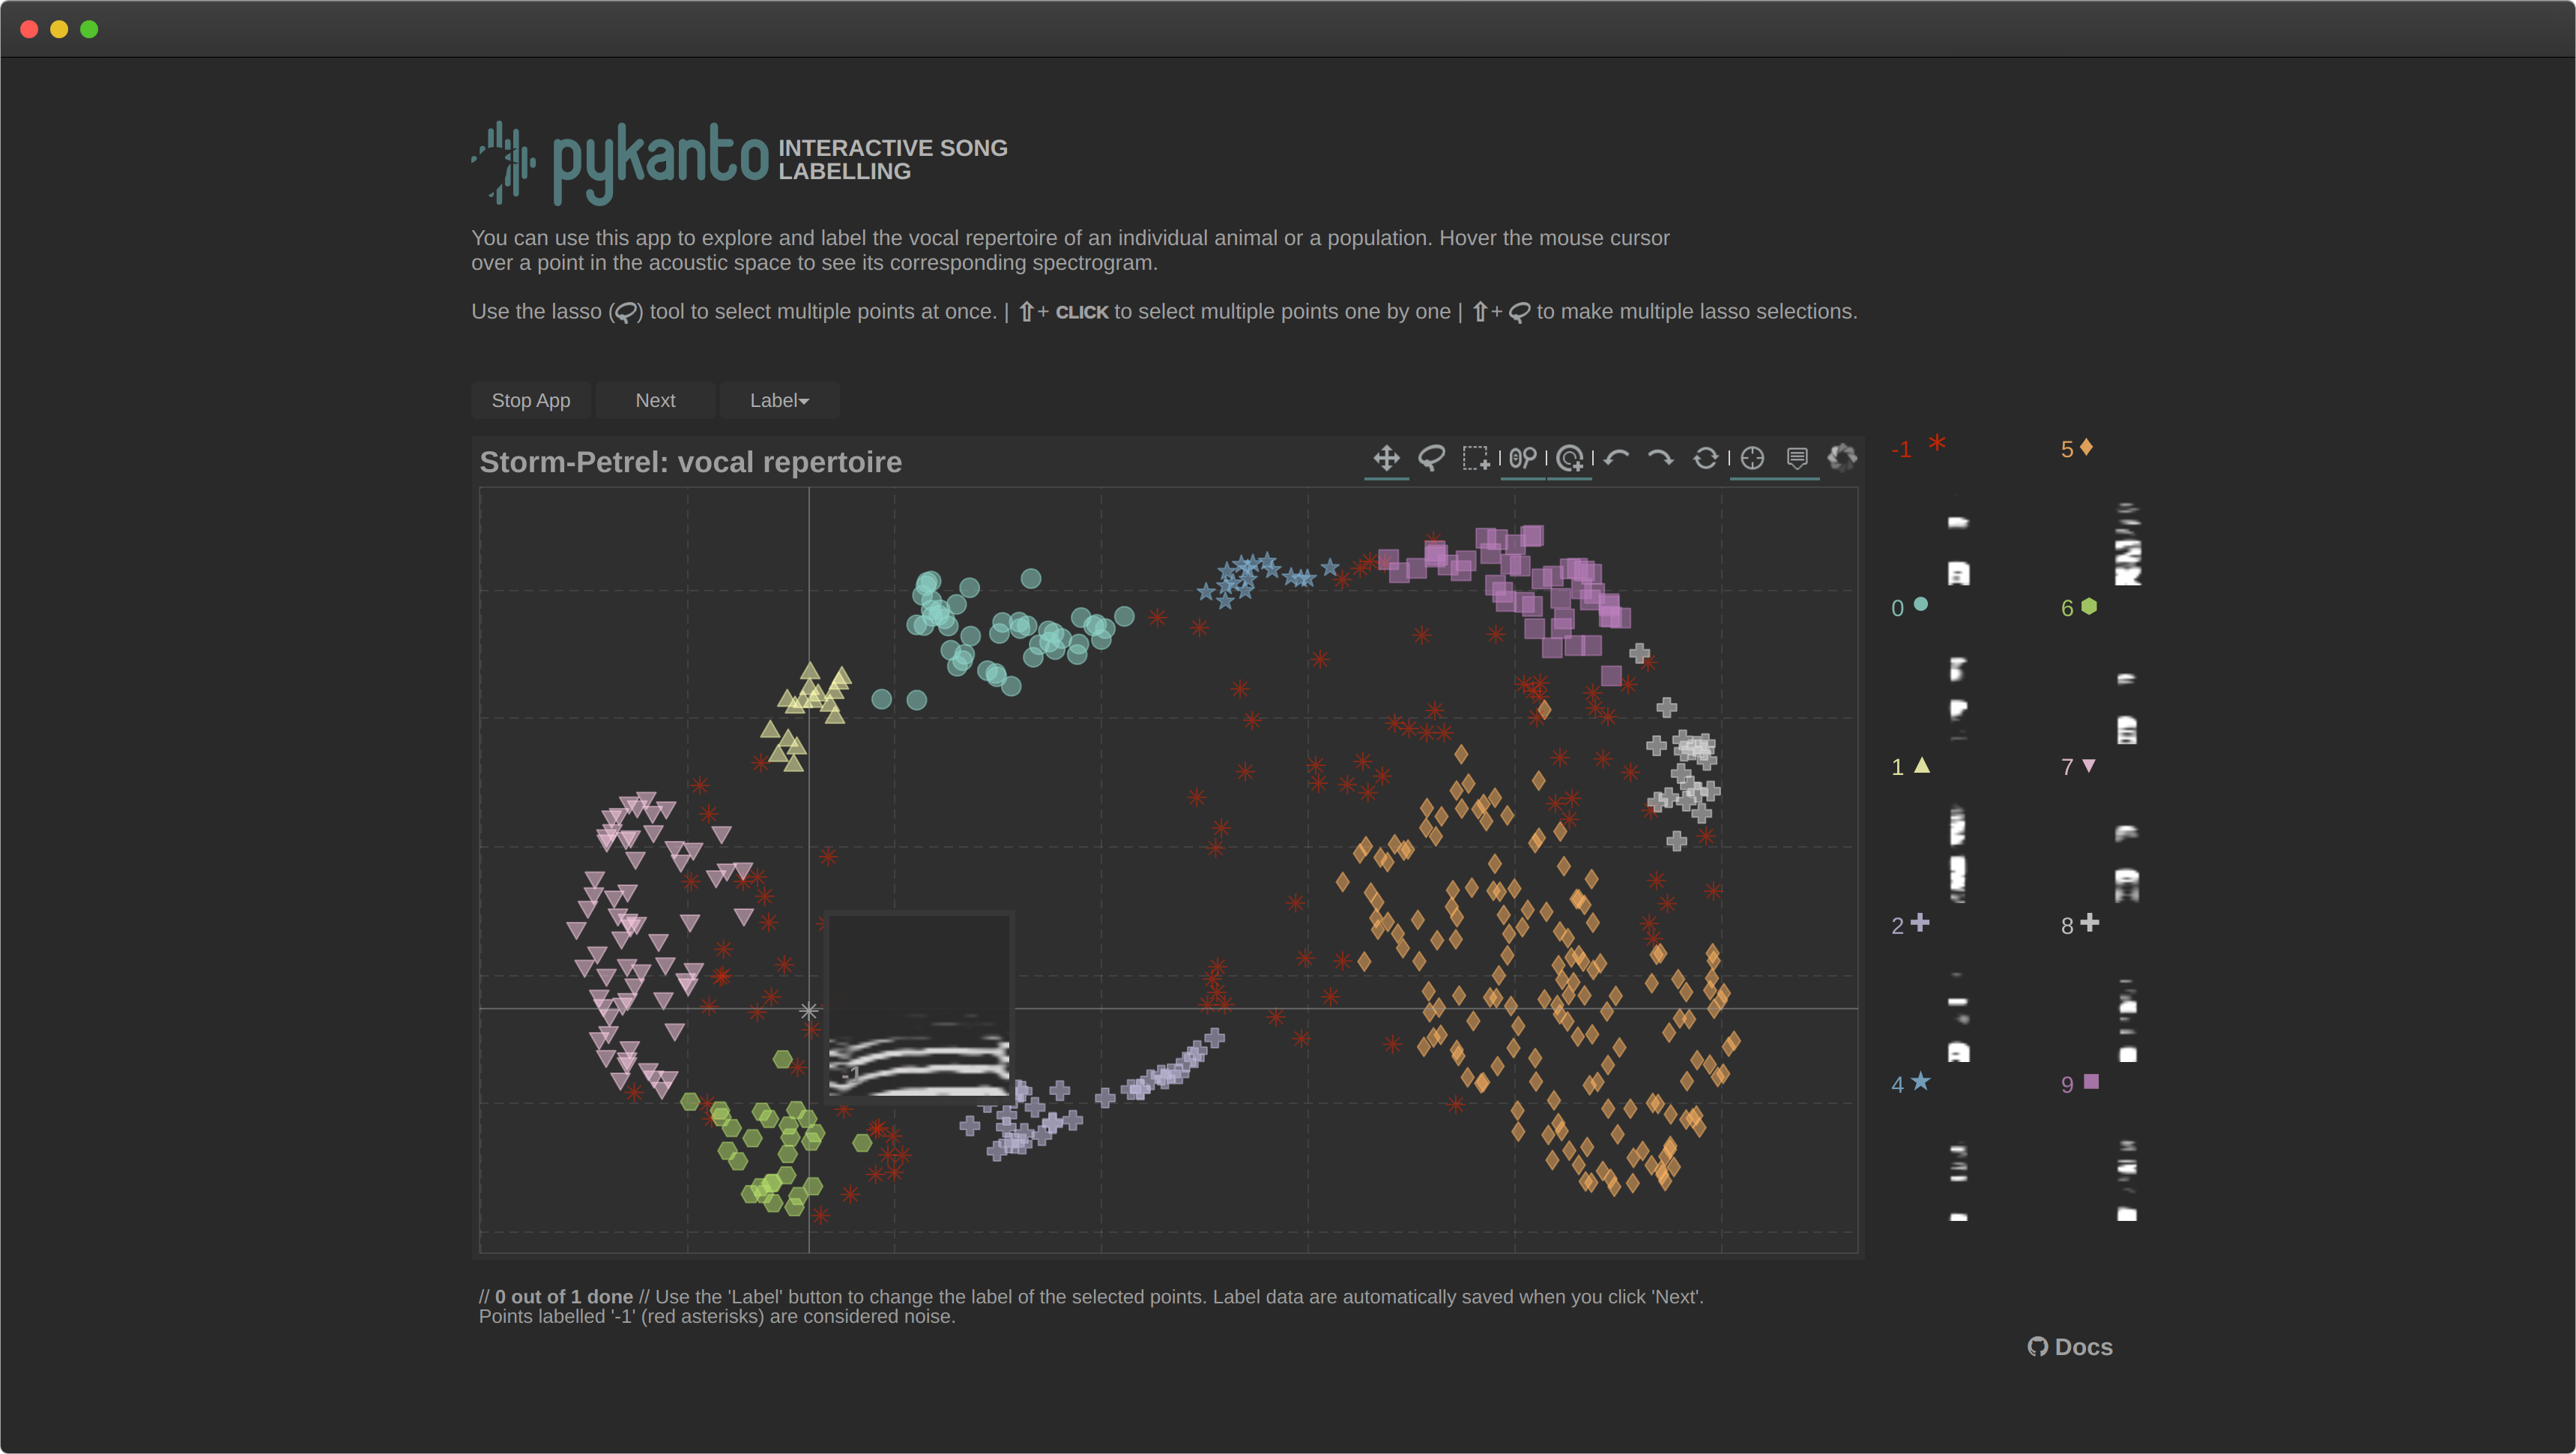
\includegraphics[width=\linewidth]{figures/chapter_2/fig1.png}
    \mycaption{Interactive web app to review and correct cluster assignment}{Interface of the interactive web app in pykanto. This app can be used to explore datasets as well as to review and correct automatically assigned class labels in bulk.}
    \label{fig:app}
\end{figure*}
%%%%%

As a response to the need for scalable and open-source tools for vocalisation
data analysis and related issues, the field of bioacoustics has recently started
to experiment with a new suite of methods based on deep-learning artificial
neural network architectures, the same that excel at, for example, computer
vision and speech recognition tasks \parencite{stowell2021}. Segmentation and
annotation pipelines based on deep neural networks have already been shown to
work well in laboratory settings, where three conditions hold: i) acoustic data
have a high signal-to-noise ratio, ii) there are orders of magnitude more
examples per vocalisation type than there are vocalisation types, and iii)
vocalisations are produced by relatively few individuals (fewer than ten to a
few tens) that do so in a stereotyped manner \parencite{coffey2019, cohen2022,
steinfath2021}. Unfortunately, none of these conditions tend to be the case in
field studies, and this creates a barrier to the adoption of new methods by
researchers working with natural populations.

This is the context in which I present \texttt{pykanto} (pronounced \textipa{pI·'kænt@U}). This software library was born of three needs, which can be summarised as follows.

\paragraph{First,} it needed to provide the infrastructure necessary to catalogue,
explore and label large acoustic datasets collected in often suboptimal field
conditions.

\paragraph{Second,} it had to serve as a flexible starting point that would allow researchers to perform both traditional analyses (such as extracting hand-picked
features from the vocalisations) and to use machine learning algorithms to learn
low-dimensional representations of the data \parencite{goffinet2021, kollmorgen2020,
morfi2021, sainburg2020}, train classifiers, or detect vocalisations in unseen
recordings \parencite{cohen2022, kahl2021, stowell2014}.

\paragraph{Third,} I wanted to build a tool that was free, open source, followed
sustainable software practises, and geared towards computational
reproducibility and transparency.

%%%%% FIG 2
\begin{figure*}
    \centering
    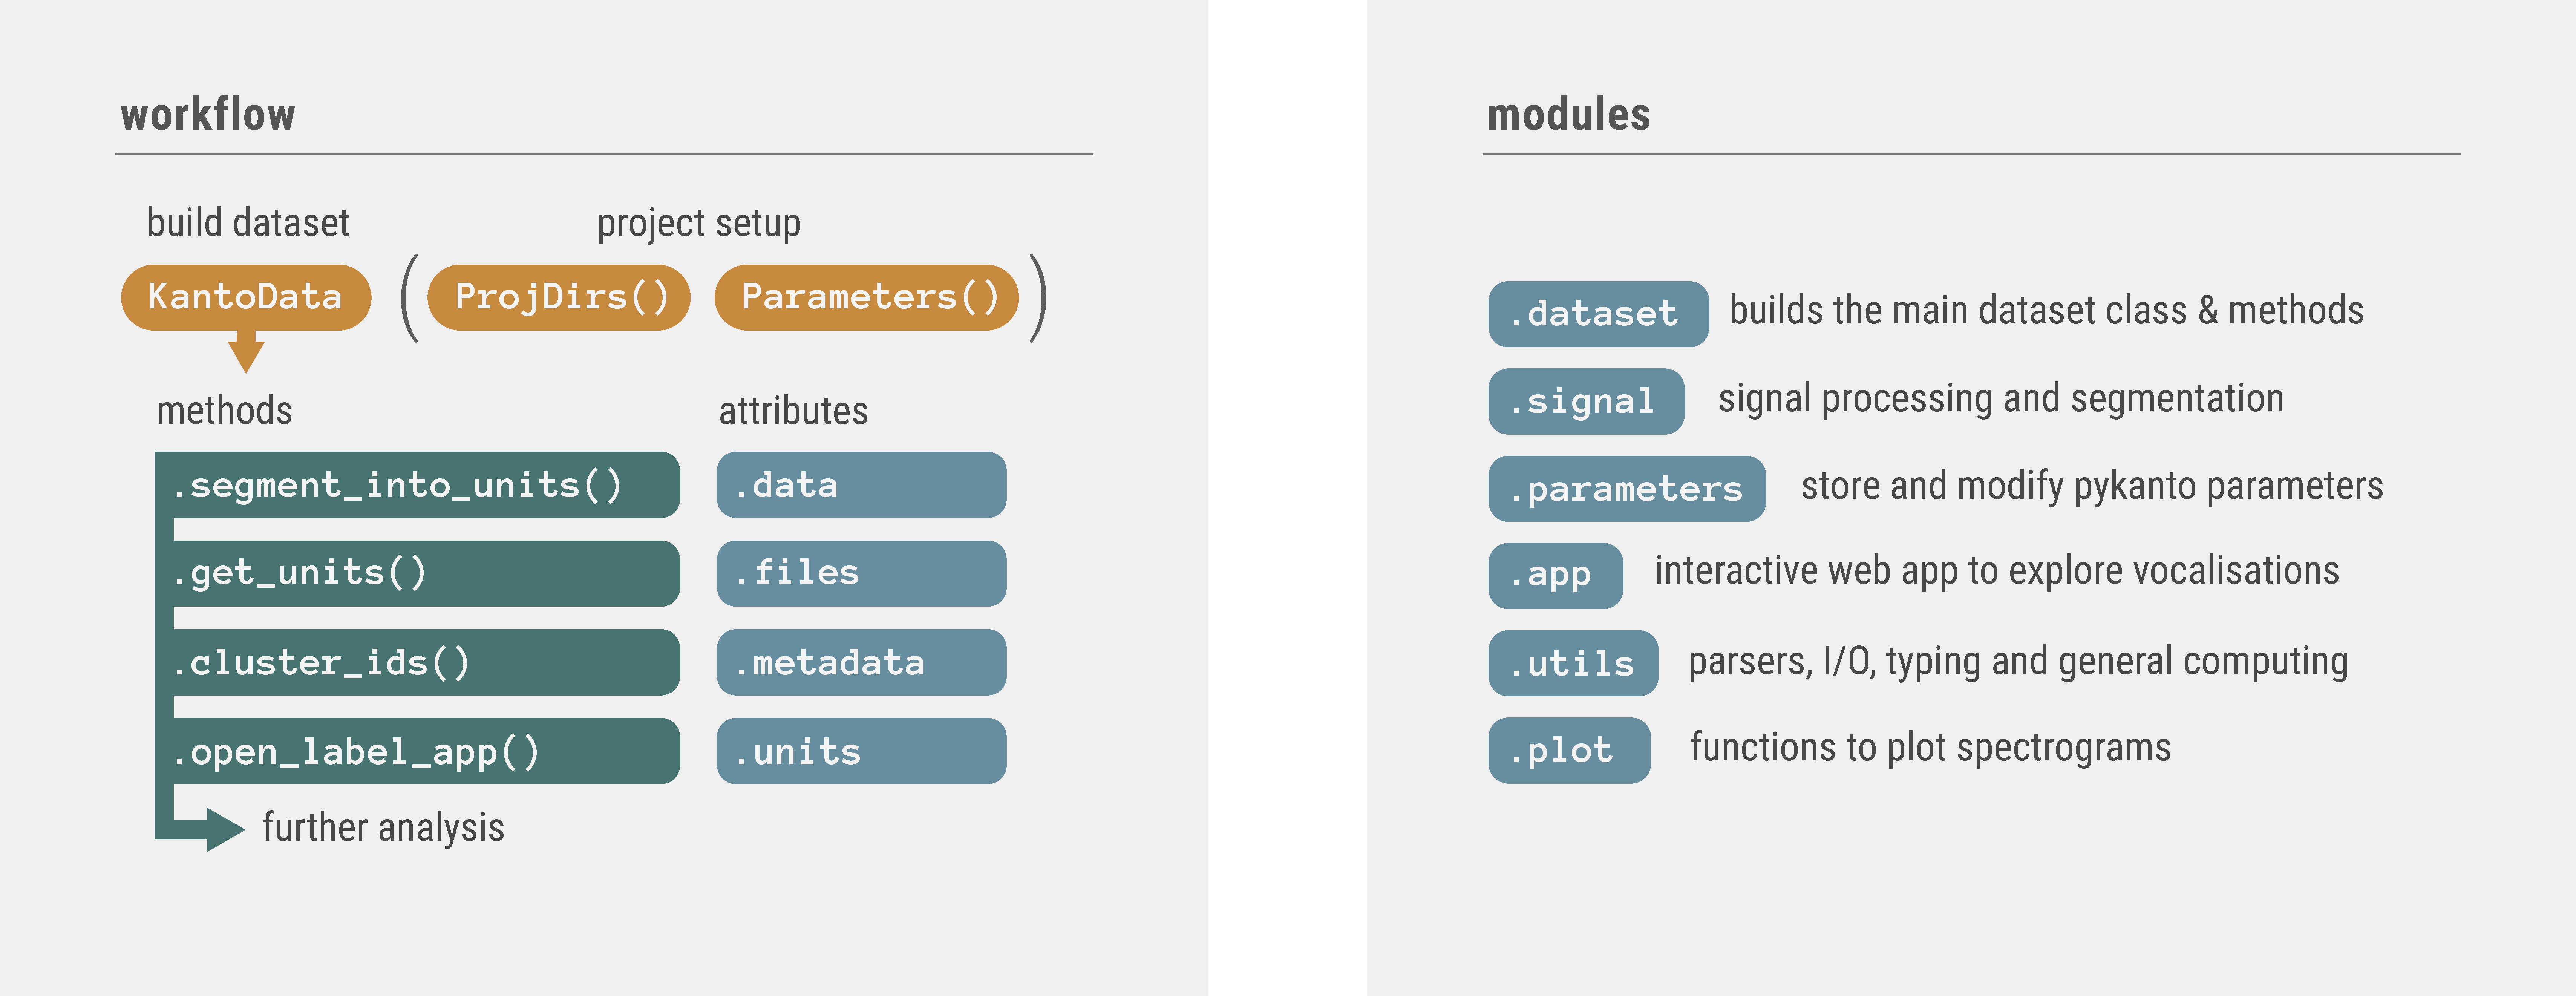
\includegraphics[width=0.6\textwidth]{figures/chapter_2/fig2.pdf}
    \mycaption{General structure of the library: main calss and modules}{\texttt{pykanto} is written around a central dataset class, \texttt{KantoData}, which provides methods to segment, visualise and label vocalisations. The library contains six modules with functions and classes to carry out common tasks in animal vocalisation analysis.}
    \label{fig:structure}
\end{figure*}
%%%%%

\section{pykanto: Implementation}

\texttt{pykanto} is a software library designed to streamline the process of
analysing animal vocalisations. It is programmed in Python and offers various
modules to assist users in their work (see \autoref{fig:structure}). The central module is
\texttt{pykanto.dataset}, which serves as a database for vocalizations and
includes methods to visualise, segment, and label them. The \texttt{pykanto.signal} module provides tools for
signal processing and creating spectrograms, while \texttt{pykanto.parameters}
contains classes and functions for managing parameters. The web application
\texttt{pykanto.app} allows users to explore and label large numbers of
vocalizations (\autoref{fig:app}) and \texttt{pykanto.plot} provides functions for
plotting spectrograms. Finally, \texttt{pykanto.utils} includes parsers, I/O
tools, custom typing, and general computing functions. The documentation for
\texttt{pykanto} is available at
\href{https://nilomr.github.io/pykanto}{\nolinkurl{nilomr.github.io/pykanto}}.

\subsection{Dependencies}

\texttt{pykanto} was written in Python 3.8 and tested in Python 3.8, 3.9 and
3.10. Its interactive web application also relies on JavaScript, HTML, and CSS.
External dependencies are automatically downloaded during package installation
(see the
\href{https://github.com/nilomr/pykanto/blob/main/pyproject.toml}{\texttt{pyproject.toml}}
file for a full list of dependencies).

\subsection{API and documentation}

\texttt{pykanto} is a well-documented code library, making it easier to use and
contribute to its development. The methods and functions in \texttt{pykanto} have clear
and concise documentation, including type annotations and descriptions of their
intended use. Its API (Application Programming Interface) reference, along with
tutorials and practical examples, can be found in the online documentation
at \href{https://nilomr.github.io/pykanto}{\nolinkurl{nilomr.github.io/pykanto}}.

\subsection{Reproducibility and open research}

\texttt{pykanto} encourages the user to create reproducible data science
projects. For example, one of its modules is dedicated to creating consistent
project structures, inspired by popular utilities such as
\href{https://github.com/cookiecutter/cookiecutter}{cookiecutter}. Using the
library requires writing simple scripts in Python, which allows every step of
the research, from data ingestion to eventual model training and reporting, to be
explicitly reproduced. The documentation includes a complete user guide with
examples of best practices.

The input and output files use open data formats, and all code is available
under the \href{https://choosealicense.com/licenses/mit/}{MIT licence} (a simple
and very permissive licence). Where applicable, we have followed the guidelines
and recommendations of the Software Sustainability Institute, a UK-based
facility dedicated to research software sustainability
(\href{https://www.software.ac.uk/}{software.ac.uk}).



Many of the processes that \texttt{pykanto} carries out are computationally
intensive, such as calculating spectrograms, performing operations on large
arrays, and running dimensionality reduction and clustering algorithms.
High-level, interpreted languages---like R or Python---are notoriously slow: where
possible, we have optimised performance by both a) translating functions to
optimized machine code at runtime using Numba \parencite{lam2015} and b)
parallelising tasks using Ray, a state-of-the-art platform for distributed
computing \parencite{moritz2018}. As an example, the \texttt{segment\_into\_units()}
function can find and segment 20.000 discrete acoustic units in approximately
16s on a desktop, 8-core machine; a dataset with over half a million (556.472)
units takes ~132s on a standard 48-core compute node. If \texttt{pykanto} detects a
suitable GPU unit and the optional dependencies are installed, algorithms such
as UMAP \parencite{mcinnes2018} switch to their GPU implementation, which provides a
15-100x speedup \parencite{nolet2021, raschka2020}. The library has a module
dedicated to making it easy for users to run their scripts in a high-performance
computing context (for example, a university compute cluster), and its
documentation includes examples of configuration and submission scripts.

\subsection{Limitations}

This final section discusses some of the main limitations of \texttt{pykanto}. Although it
will hopefully offer a flexible solution for researchers, it is also limited in
important ways.

\paragraph{Limitation 1} Vocalisation unit segmentation via the very simple amplitude
thresholding algorithm will not work well with species whose vocalisations vary
greatly in amplitude, or with very noisy datasets. In those cases, and depending
on data volume,  segmentation might better be performed either manually or in a
semi-automated way. For example, one could use \textit{chipper}
\parencite{searfoss2020a} or train a neural network like TweetyNet,
\parencite{cohen2022} on a manually annotated subset of the data.

\paragraph{Limitation 2} \texttt{pykanto} has been tested on species that produce
vocalisations made up of a small or moderate number of different but distinct
elements (variously referred to as notes or syllables). It will be useful for
researchers working with any species, but the automatic part of the clustering
process will work increasingly poorly with those that have a large number of
very variable elements. This is true of any clustering method: they will fail or
produce spurious results if variation in the data is continuous.

\paragraph{Limitation 3} The library does not include methods to train models intended to
find analysable vocalisations in long recordings of entire soundscapes. This is
a particularly challenging problem \parencite{priyadarshani2018} without a universal
solution. However, \texttt{pykanto} can be used to generate and organise the training
data required by these models \parencite{kahl2021, stowell2019, stowell2014}, and to
work with their output annotations.

\paragraph{Limitation 4} \texttt{pykanto} is intended as a flexible solution for managing
and preparing animal vocalisation data for further analysis. It provides tools
that can save researchers a great deal of time while making analysis pipelines
more reproducible. However, it does not implement any specific analysis or
feature extraction methods, since these will vary greatly by use case. This
means that researchers using the library as part of their work will need to
either have or develop familiarity with bioacoustic analysis and scripting in
Python.

\section{Using pykanto: can individual birds be identified from their songs?}

I now provide a worked example of how \texttt{pykanto} can be used to help answer real research questions about vocalisations---bird song in this case:

\subsection{Introduction}

Great tits are small, short-lived birds (average lifespan: 1.9 years) that sing
acoustically simple yet highly diverse songs. In Wytham Woods, Oxfordshire (UK),
a population of these birds has been the focus of a long-term study that is now
in its 75th year. For the past three years, I have recorded the song repertoires of
hundreds of individual males when they sing close to their nest before their
partner begins laying. With the help of these data, we are trying to answer
questions about song learning and cultural change in natural populations.

To do this we first need to know which individuals are present in the breeding
population for the first time, and which were already around in previous years.
However, individual survival over the winter months is low and detection by
traditional means---such as mist-netting or identification in the nest---is
imperfect. So we would first like to test whether individual birds can be
identified based on their songs alone, and then quantify how much variation in
song types occurs within and between years.

Our example dataset consists of 5293 songs from 12 males that were known (from
physical recaptures) to be present in the breeding population in two different
years, 2020 and 2021. Although this is a small subset of our data, it is large
enough that it would still take weeks to process and analyse using traditional
methods. We demonstrate the use of \texttt{pykanto} to a) organise, segment and label the
dataset, and b) prepare it so that we can train a deep neural network to
recognise the bird's song types. The entire process, which takes under an hour to complete,
can be computationally reproduced using its
\href{https://github.com/nilomr/pykanto-example}{dedicated
repository}. The repository includes
raw data, auxiliary scripts and detailed instructions. Below is a short
narrative description of the process.

\subsection{Data collection}
Most great tits in our population nest in nest boxes with known locations. Every year, fieldworkers record the identities of breeding males and females, clutch initiation and egg-hatching dates, clutch size, and fledgling success using standardized protocols. A significant number of birds in the population are fitted with a unique British Trust for Ornithology (BTO) metal leg ring as nestlings or adults. During the breeding season (March to June), great tit pairs are socially monogamous and protect territories around their nest boxes \parencite{hinde1952}.

We collected data during the breeding seasons of 2020 and 2021, from early April to late May, using a dense sampling design with multiple recorders placed in nest boxes throughout the study site. Fieldworkers checked every nest box in the study site at least once a week before and during egg laying, which can last from one to 14 days \parencite{Perrins1965}. Once a nest box was believed to be in use by a great tit, we placed an autonomous sound recorder in its vicinity, either in the same tree or in a suitable neighbouring tree. We left each recorder in the same location for at least three consecutive days before moving it to a different nest box. Throughout the recording period, we relocated 20 recorders every day.

We used 60 AudioMoth recorders \parencite{hill2019} in 2021 and 30 in 2020, which were housed in waterproof custom-built enclosures. Recording began about an hour before sunrise (from 05:36 to 04:00 UTC during the recording period) and consisted of seven 60-minute recordings with a sample rate of 48 kHz. Since the recording process was automated, there is a possibility that some of the songs recorded in the immediate vicinity of a given nest box do not belong to the focal bird. To reduce the risk of false positives, we discarded recordings with more than one vocalizing bird, unless one was distinctly louder than the others. We also discarded all songs with a maximum amplitude below $-16 dB$, calculated as $20\log_{10} \left (\frac{A}{A_{0}}\right )$, with $A = 5000$ and $A_{0} = 32767$ (the maximum value for 16-bit digital audio). This threshold was determined from the observation that, in cases where we had simultaneous recordings of close neighbours from the centres of their respective territories, an amplitude cutoff greater than 4000 always separated a focal bird from its neighbours. It should be noted that these values are not calibrated and are relative to the recording equipment and settings used, as well as other factors such as sound directionality and vegetation cover.

\subsection{Running the analysis}
\subsubsection{Installation}

\texttt{pykanto} can be used outside a virtual environment, but this is not encouraged.
Using clean environments for each project will allow you to avoid dependency issues. Once inside a new environment with Python 3.8 or above, you can
install \texttt{pykanto} by simply running \texttt{pip install pykanto}, then install the
package containing this example. See detailed installation and use instructions
in the \href{https://github.com/nilomr/pykanto-example}{\texttt{.README}}.

\subsubsection{Creating a new project and dataset}

Our first step will be to define a directory structure for our project and a
\texttt{ProjDirs} object to hold everything together. Then, we can test and set
adequate parameters for our dataset. These include things like low- and high-cut
filters, spectrogram settings, amplitude thresholding, and whether the analysis
will be carried out at the song or note level. The data folder in the project
already contains \texttt{.wav} audio files and their corresponding
\texttt{.json} with annotations, so we can create a \texttt{KantoData} instance:
this will be our database.

\subsubsection{Segmenting songs and using the interactive app}

Then, using the \texttt{.segment\_into\_units()} method, we find segment onsets,
offsets, unit and silence durations and add them to \texttt{KantoData.data}, the
main data frame in our database object. At this point, we could already carry
out most of the analyses common in the bird song literature, for example, by
extracting some simple acoustic parameters from the segmented data. Instead, we
want to preserve all the temporal and spectral information that is available in
the spectrograms to train a more accurate classifier.

The next step is to compute and store spectrograms for each unit under
examination, and then reduce their dimensionality and group them into clusters.
This can be achieved by using the \texttt{.get\_units()} and \texttt{.cluster\_ids()} methods, which
employ algorithms such as UMAP \parencite{mcinnes2018} and HDBSCAN
\parencite{mcinnes2017}. Afterwards, we can launch the interactive web app by
calling \texttt{.open\_label\_app()}. Using this app, we can review the automatic labels
for up to tens of thousands of vocalisations at once, splitting or combining
clusters as needed. Once completed, we will have a fully annotated dataset, which
can be divided into training and testing sets and exported as labelled
spectrograms using \texttt{pykanto}. 



%%%%% FIG 3
\begin{figure*}
    \centering
    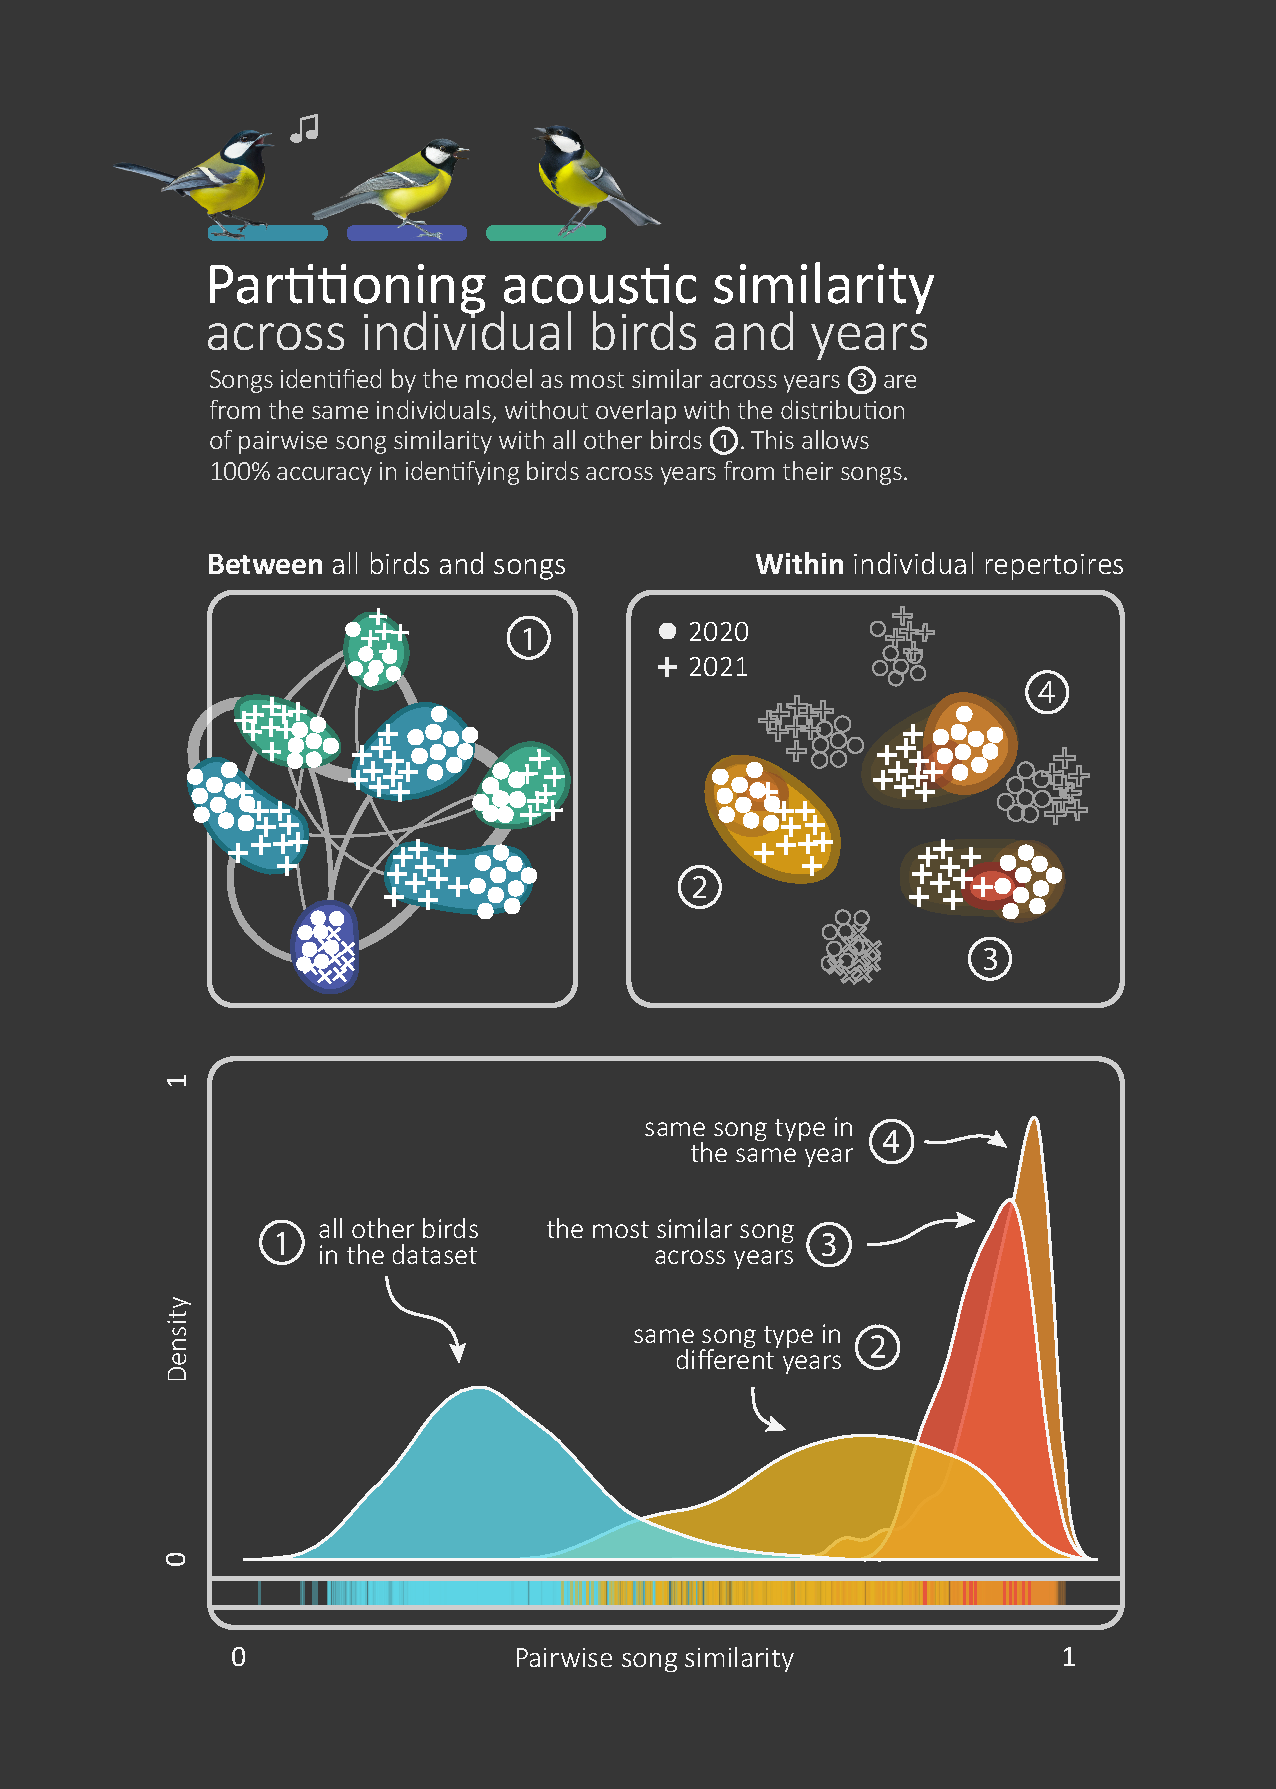
\includegraphics[width=\linewidth]{figures/chapter_2/fig3.pdf}
    \mycaption{Partitioning acoustic similarity between and within birds}{(From left to right and top to bottom.) First, we calculate the pairwise similarity between the songs of all birds, which provides a baseline distribution of similarity in the population (1). Then, we compare songs from the same bird in different years (2), find the pair of songs that are most similar across years (3), and compare songs within the same year (4). The probability density estimates in the bottom panel show how pairwise similarities in (3) allow us to re-identify birds across as they do not overlap with any other birds (1).}
    \label{c2_fig:results}
\end{figure*}
%%%%%

\subsubsection{Training a convolutional neural network classifier}
Our goal is to generate compressed representations of songs that can facilitate comparisons and identification of those sung by the same individual, even in the presence of variations in performance and noise. To do this, we can train a model to distinguish between different song types, which are categorically distinct within individual song repertoires, without providing the model with information about who sang them. 

In this example, we use weights from a pre-trained ResNet50 backbone \parencite{he2015} and gradually unfreeze the earlier layers of the network during training. By doing so, we can fine-tune the network to attain better performance in our task, while still benefiting from the weights learned on a much larger dataset \parencite{zhuang2021}. 

The distribution of song sample sizes per individual approximately follows a
power law, so there is a very large amount of data for a few birds and very
little for most. This imbalance of data is problematic for learning algorithms, as they may develop a bias toward larger classes and perform poorly on rarer ones. There are different ways to deal with this \parencite[see, e.g.,][]{krawczyk2016, thabtah2020}; however, to keep things simple, here we will just undersample majority classes so that all birds have the smallest common sample size for each song type.

Background noise can also bias our analysis. Each bird's acoustic environment is unique, and the network may learn to distinguish between songs based on this noise rather than the signal of interest. To address this issue, we remove most background noise by thresholding the spectrograms, taking advantage of the difference in amplitude between the focal bird singing near the recording and its acoustic background. Additionally, we apply a series of data augmentation techniques during the training process to prevent over-fitting and ensure that the algorithm does not memorise irrelevant or highly variable elements. These techniques include semi-random cropping in the time domain, blurring and sharpening, random erasing of parts of the spectrogram, and contrast and brightness changes. After training the model, we can verify that background noise is not causing bias by checking whether songs recorded in the same location are classified as more similar than expected by chance. In addition, we can create class activation maps to identify the regions of the spectrograms used by the model to generate predictions.

Once the model is trained, we can assess its ability to classify unseen songs drawn from the held-out dataset, which can reach an accuracy of around 92\%. As described below, most of the remaining 8\% can be attributed to confusion between the same song types sung by the same birds in different years. 

Finally, we can use the model to extract a compressed representation of each song in the entire dataset. This is achieved by passing each song through the trained network and obtaining the output from the last hidden layer. This output consists of a feature vector that captures the most relevant information to distinguish between different types of songs; these feature vectors can then be used to determine whether two songs are very similar. In our case, we do this by taking the inverse of the cosine distance between each pair to build a similarity matrix.

The repository that supports this paper contains a streamlined way of doing this using PyTorch (\citeyear{pytorch2019}) and PyTorch Lightning (\citeyear{pytorchlightning2019}) that can be easily adapted for use with other datasets.


\subsection{Results \& Discussion}

After calculating the similarity scores between all pairs of songs, we grouped them according to song type, the bird that sang them, and the year they were sung. For each bird in the first year, we identified the individual who sang the song with the highest similarity to any within its repertoire during the following year. We found that we were able to successfully identify the correct bird in all cases, even though the baseline probability was only 2.27\% (1 out of 44 song types). This suggests that we would have been able to re-identify the individuals even if they had not been observed or captured again.

As shown in \autoref{c2_fig:results}, the highest similarity values correspond to
comparisons of the same song types within years and birds. The similarity
between the same song types sung by the same bird across different years is
consistently higher than that between different birds, even when some song types were shared by individuals: this means that individual vocal signatures are
at least partly maintained across their lifespan.

The conclusions drawn from this analysis are limited by the small size of the
dataset: including more birds would likely lead to noisier results, as it increases the chances of finding a second bird with even more similar songs. Nonetheless, in
combination with other information (such as spatial location), they might allow
high-confidence identification of individuals between years without physical
capture.

This example illustrates how \texttt{pykanto} can be used to help address a
specific research question. The model-based feature vectors used to describe each song
can be imported back into the \texttt{KantoData} database as a new column, enabling a
wide range of research possibilities while maintaining a clear project
structure.

\section{Data availability}

We distribute \texttt{pykanto} with three sample datasets that are used to run unit tests
and as examples in the documentation \parencite{nilo_pykanto_2023}.

\paragraph{Great tit songs} 20 songs recorded from male birds during the dawn chorus in a
population in Oxford, UK. Recorded by the author and accessible at \href{https://github.com/nilomr/pykanto/tree/main/pykanto/data/segmented/great_tit}{pykanto/data/great\_tit}.

\paragraph{European storm-petrel purr songs} Two males singing from burrows in the Shetland
and Faroe islands. Source: \href{https://xeno-canto.org/46092}{XC46092} (©
Dougie Preston), \href{https://xeno-canto.org/663885}{XC663885} (© Simon S.
Christiansen). Under
\href{https://creativecommons.org/licenses/by-nc-nd/2.5/}{CC BY-NC-ND 2.5
licence}.

\paragraph{Bengalese finch songs} Recordings from 2 isolated Bengalese finches. Originally
published in Tachibana, Koumura and Okanoya \parencite{tachibana2015}, data can be
accessed at \href{https://osf.io/r6paq/}{OSF}.\par

They can be found under \texttt{pykanto/data} when you install the package, as well as in the \href{https://github.com/nilomr/pykanto}{GitHub repository}.

\paragraph{}Additionally, the worked example in this article uses 5293 songs from male great tit songs recorded by the author between 2020 and 2021 in Wytham Woods, Oxfordshire, UK. They are available from \href{https://github.com/nilomr/pykanto-example/tree/main/data/segmented/pykanto-example}{pykanto-example/data} on GitHub, along with detailed metadata \parencite{nilo_pykanto_example_2023}.

\section{Code availability}

The latest version of \texttt{pykanto} is available from PyPI (\texttt{pip install
pykanto}) and its source repository (\href{https://github.com/nilomr/pykanto}{github.com/pykanto}). See the repository for detailed installation instructions.

\texttt{pykanto} and the example in this article rely on the following open-source scientific
libraries or tools: numpy \parencite{numpy2020}, scipy \parencite{scipy2020}, pandas
\parencite{pandas2023}, numba \parencite{lam2015}, pytorch \parencite{pytorch2019},
torchvision \parencite{torchvision2016}, pytorch lightning
\parencite{pytorchlightning2019}, tqdm \parencite{tqdm2019}, ray \parencite{moritz2018},
soundfile \parencite{bechtold2022}, umap \parencite{mcinnes2018},  joblib
\parencite{joblib2020}, hdbscan \parencite{mcinnes2017}, seaborn \parencite{Waskom2021},
scikit-image \parencite{scikitimage2014}, librosa \parencite{mcfee2015}, bokeh
\parencite{bokeh2018}, ujson \parencite{ujason2023}, psutil \parencite{psutil2023}, attrs
\parencite{schlawack2019}.

\section{Acknowledgements}

I thank Ben Sheldon and the Sheldon lab for their support and
patience. Ben Sheldon, Carys Jones and Andrea Estandia provided useful comments on a draft of this
manuscript. Carys Jones and Antoine Vansse tried early versions of the
interactive app in \texttt{pykanto} and provided valuable feedback.

Some of the methods in \texttt{pykanto} are directly inspired by or adapted
from \cite{sainburg2020}. I have indicated where
this is the case in the relevant method's docstring. The dereverberation
function is based on code by Robert Lachlan that is part of Luscinia
\parencite{lachlan2016a}, a software for bioacoustic archiving, measurement and
analysis. Please consider citing these two publications if you use
\texttt{pykanto} on your own projects.

I have learnt a great deal about packaging and developing in Python by browsing
the structure of existing open source projects, for example some by David
Nicholson (\href{https://github.com/NickleDave/NickleDave}{@NickleDave}). I only
became aware of \href{https://github.com/vocalpy}{VocalPy}, a project that aims
to "develop an ecosystem of interoperable packages" for
"computational vocal communication and learning research" when I had
already written most of \texttt{pykanto}, but eventually, I would like to make it
compatible with it: standardisation is direly needed in the field and I don't
want to contribute to the chaos.

This work was supported by a Clarendon-Mary Frances Wagley Graduate Scholarship
and an EGI scholarship to Nilo Merino Recalde, and made use of the University of Oxford Advanced
Research Computing facility \parencite{richards2015}.

\section{Conflict of interest}

The author declares no conflict of interest.

\section{Author contributions}

Nilo Merino Recalde wrote the software library and its documentation, collected the data,
conducted the analyses, and wrote the manuscript.

\renewcommand{\cleardoublepage}{}
\renewcommand{\clearpage}{}
\printbibliography

    \end{multicols} % end one-column layout
    \onecolumn




% Chapter 3: dataset =================


\runningauthor{Merino Recalde \textit{et al}., 2023 }
% \runningtitle{The Wytham Woods great tit song dataset}
\fancyhead[LE]{\sffamily\color{black50}\thepage\hspace{2em}The Wytham Woods great tit song dataset}
\clearpage{\pagestyle{empty}\cleardoublepage} % empty page before chapter
\onecolumn % start one-column layout for chatper 4

    \chapter{A densely sampled and richly annotated acoustic dataset from a wild bird population}
    \vspace{10pt}
    \thispagestyle{empty}  % remove page number 
    {\normalfont\sffamily\raggedleft
    {
        Nilo Merino Recalde \orcidlink{0000-0003-3903-1288}\textsuperscript{1,$\ast$}, 
    Andrea Estandía \orcidlink{0000-0002-3895-2141} \textsuperscript{1}, 
    Loanne Pichot\textsuperscript{2},\\
    Antoine Vansse\textsuperscript{2},
    Ella F. Cole \orcidlink{0000-0002-2689-946X}\textsuperscript{1}, 
    and Ben C. Sheldon \orcidlink{0000-0002-5240-7828}\textsuperscript{1}\par
    \vskip 0.7em

    {\small\textsuperscript{1}Edward Grey Institute, Department of Biology, University of Oxford, Oxford, UK\\
    \small\textsuperscript{2} École Normale Supérieure de Lyon, Lyon, France\par}

    \small\textsuperscript{$\ast$}Corresponding author: \href{mailto:nilo.recalde@biology.ox.ac.uk}{nilo.recalde@biology.ox.ac.uk}

    } }

    \myabstract{
        \noindent We present a high-resolution, densely-sampled dataset of wild bird songs collected over multiple years from a single population of Great Tits (\textit{Parus major}) in the UK. The dataset includes over 1,100,000 individual acoustic units from 109,963 richly annotated songs, sung by more than 400 individual birds, and provides unprecedented detail on the vocal behaviour of wild birds. Here, we describe the data collection and processing procedures and provide a summary of the data. We also discuss potential research questions that can be addressed using this dataset, including behavioural repeatability and stability, links between vocal performance and reproductive success, the timing of song production, syntactic organisation of song production, and song learning in the wild. We have made the dataset and associated software tools publicly available with the aim that other researchers can benefit from this resource and use it to further our understanding of bird vocal behaviour in the wild.}

    {\small\textsf{\textbf{Keywords:} animal culture; bird song; demography, cultural evolution}}

    \vspace{.5cm}

\begin{multicols}{2} % start one-column layout
    \section{Introduction \& background}
\lettrine[lines=2]Despite a long history of scientific interest from disciplines as diverse as behavioural ecology, neurobiology and physiology, there is still much to learn regarding the evolution and function of animal vocalizations. Ongoing research covers a wide range of topics, including speech recognition and language evolution in humans, animal welfare, and even fish vocal communication. The study of animal vocalizations offers valuable insights into the intricacies of social interactions and reproductive strategies. They frequently convey crucial information about an individual's condition and identity \parencite{lehmann2017, linhart2019}, the cohesion of social groups, and the structure of social hierarchies \parencite{bell2010, engesser2022, radford2007}. Additionally, animal vocalizations play a substantial role in the formation of social bonds, the selection of mates, and the provision of parental care \parencite{behr2004, gerhardt1991, pitcher2010, roulin2001}.

For those interested in social learning and cultural evolution, animal vocalizations, particularly those of birds, have long been a focus of research. This interest dates back at least to the pioneering work of Marler and Thorpe with Chaffinches \textit{Fringilla coelebs} and White-crowned Sparrows \textit{Zonotrichia leucophrys} \parencite{marler1964, Marler1962, marler1952, thorpe1958}, which paved the way for what continues to be a thriving field today (see \cite{mets2019, riebel2015, williams2021, youngblood2022}). In addition, and from a more mechanistic point of view, they offer a window into the physiological and neural mechanisms underlying vocal production and perception, as well as the consolidation of memories and motor coordination, to name but a few \parencite{davenport2023}. 

Beyond their fundamental scientific importance, animal vocalizations have practical applications in various fields. For example, there is increasing recognition of their potential as a non-invasive tool for monitoring populations. By analysing entire soundscapes, researchers can gather crucial information about population dynamics, species distribution, and the presence of rare or elusive species \parencite{kahl2021, sethi2020, sugai2019}.

However, despite the growing interest in animal vocalizations and their potential applications, publicly available data from wild populations are still scarce---with the \href{https://xeno-canto.org/}{xeno-canto} community science project as a prominent exception, focusing primarily on sparse recordings of most of the world's bird species rather than dense sampling of populations within the same species. This can severely limit researchers' ability to ask questions that require large datasets to answer, such as those about social learning, vocal development, large-scale cultural diversity, and the syntactic structure of animal vocalizations \parencite{aplin2019, kollmorgen2020, lachlan2018, sainburg2019}. Indeed, while controlled laboratory settings allow researchers to track vocal development and production in minute detail, it is much harder to obtain finely-grained data from animals in their natural habitats. The process of collecting such data can be quite demanding and requires significant time, technical expertise, and resources: this includes both data collection itself and the subsequent processing of acoustic data files.

A second limitation arises after data have been collected, due to (i) researchers' understandable focus on specific, often narrowly defined questions, (ii) practical constraints, and (iii) scientific cultural norms that have not encouraged data-sharing. Combined, these factors often lead to a tendency of not publishing or only partially publishing the data collected during research. This lack of data sharing can hinder scientific progress and make it difficult to reproduce research findings \parencite{jenkins2023, powers2019, reichman2011, wilkinson2016}; hence, we argue that there is great intrinsic value in publishing fully curated acoustic datasets. If this practice becomes widespread, it would allow scientists to explore a broader range of research questions, improve reproducibility, and facilitate the validation of findings across different studies and populations \parencite{hersh2023, powers2019}.

%%%%% FIG 1: SUMMARY
\begin{figure*}[htbp]
    \centering
    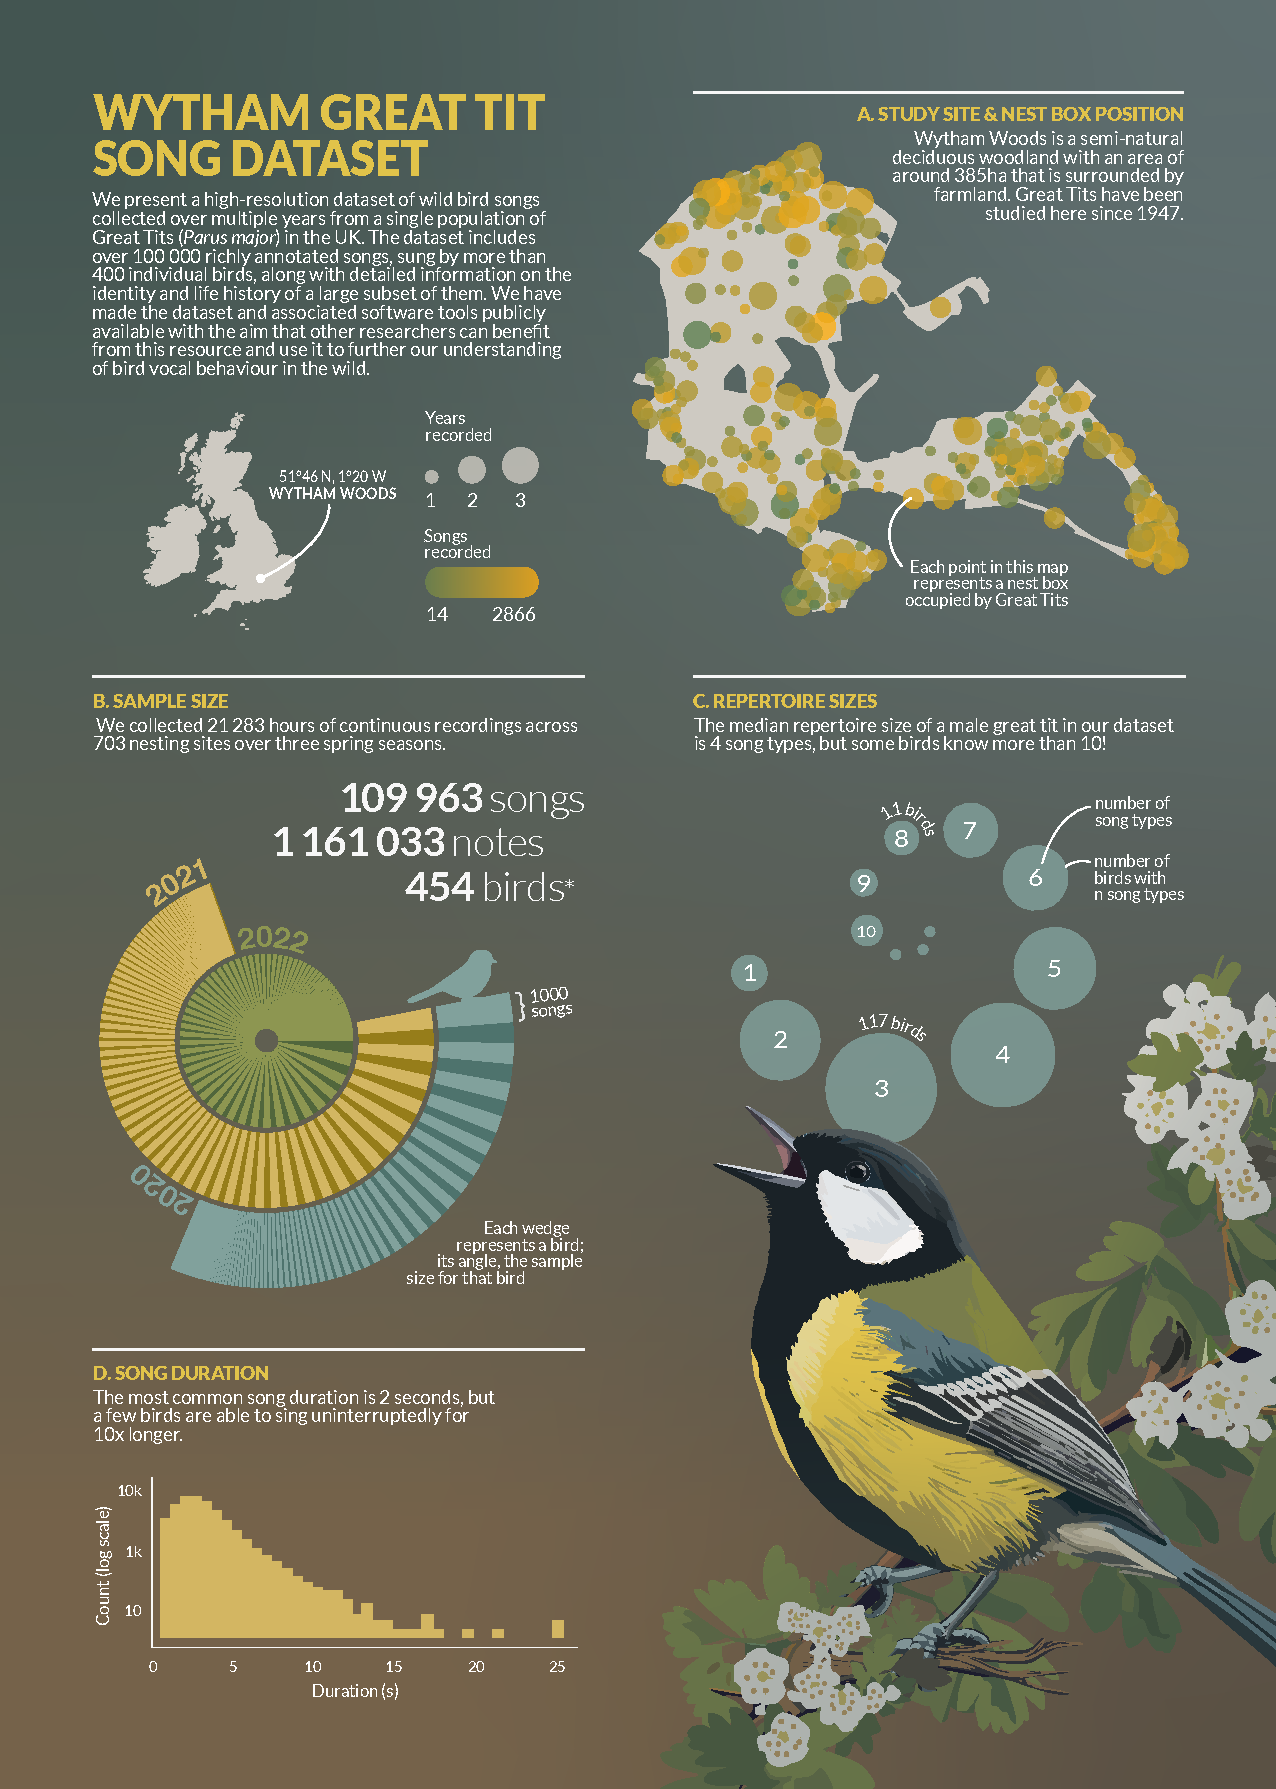
\includegraphics[width=\linewidth]{figures/chapter_3/FIG1-AB.pdf}%
    \mycaption{Description of the study site and dataset}{(A) Map of the study site and sample locations, (B) total sample sizes for each bird and year, (C) distribution of repertoire sizes, and (D) distribution of song lengths. *The exact number of individual birds is not known exactly.}
    \label{c3_fig:summary}
\end{figure*}
%%%%%


In line with this perspective, we present a comprehensive dataset of wild bird songs recorded from a single population of great tits (\textit{Parus major}) in Wytham Woods, Oxford, UK. We collected 21,283 hours of continuous recordings across 703 nesting sites over three spring seasons, which resulted in the annotation of over 1,100,000 notes or acoustic units from more than 100,000 songs (see below for definitions of these terms), sung by approximately 400 different male great tits. Among these birds, we have detailed information on the identity and life history of 242 individuals, including 50 that were recorded in multiple years. This information includes the time and location of breeding attempts, clutch size, number of fledglings, age of the bird, and basic morphological traits. For birds born in the population (106, or 43\% of the total), we also include details such as birthplace, postnatal dispersal distance, mother, and social father. 

To complement the song recordings, we have prepared extensive metadata for each of the more than 100,000 songs. This includes details such as the onset and offset times of each note within the song, a song type label, and the time of recording. We also provide the time of the first song during dawn. Finally, we augment the dataset by providing embeddings of each song, which are vector representations derived from a deep metric learning model specifically trained on this dataset. These can be used to identify individuals and in tasks that require similarity judgements.

Great tit song has been the subject of extensive research activity (see, for example, \cite{lambrechts1990, lind1996, rivera-gutierrez2010a, rivera-gutierrez2010, rivera-gutierrez2011, slagsvold1994, Ritschard2012}). Research conducted within the Wytham Woods population, in particular, has given rise to many influential ideas and insights into bird singing behaviour. These include investigations into neighbour interactions, song matching and the connection between song repertoires and reproductive success \parencite{mcgregor1981, mcgregor1983, mcgregor1989}, the dynamics of song learning from neighbouring individuals and the acquisition of distinct song types \parencite{mcgregor1989, mcgregor1982b}, as well as the role of song repertoires in maintaining territories and reducing listener habituation \parencite{krebs1976, krebs1978}, the functions of dawn song \parencite{kacelnik1983, mace1987}, and the influence of spatial factors and movement on song culture \parencite{fayet2014}. We hope that this dataset---which is, to the best of our knowledge, the largest publicly available collection of bird songs from a single wild population---will contribute to that effort by providing valuable insights into a range of scientific questions, including behavioural repeatability and stability, links between vocal performance and reproductive success, the timing of song production, the syntactic organization of song production, and song learning in the wild.

What follows is a detailed description of the data collection and curation process and the resulting dataset, together with some discussion around potential uses of data presented in this format.

\section{Data collection}
\subsection{Study system \& fieldwork}

Great tits are small, short-lived birds---average lifespan: 1.9 years---that sing acoustically simple yet highly diverse songs. During the breeding season, from March to June, great tit pairs are socially monogamous and defend territories around their nests \parencite{hinde1952}. In Wytham Woods, Oxfordshire, UK (51\degree46 N, 1\degree20 W), a population of these birds has been the focus of a long-term study since 1947 \parencite{lack1964}. Wytham Woods is a semi-natural predominantly deciduous woodland that spans an area of approximately 385 hectares and is surrounded by farmland. Most great tits in this population breed in nest boxes with known locations (see map in \hyperref[c3_fig:summary]{Figure \ref*{c3_fig:summary}}), and the majority of individuals are marked with a unique British Trust for Ornithology (BTO) metal leg ring as nestlings or adults. 

We collected data from late March to mid-May during the breeding seasons of 2020, 2021, and 2022. Every year, fieldworkers checked each of the 1018 nest boxes at least once a week before and during the egg-laying period, which typically lasts from one to 14 days \parencite{Perrins1965}, and recorded the identities of breeding males and females, the dates of clutch initiation and egg hatching, clutch size, and fledgling number and condition under standardized protocols. We found the first egg date by assuming that one egg is laid every day and counting back from the day of observation. In cases where we did not observe the chicks on the day of hatching, the actual hatching date was determined by assessing the weight of the heaviest chicks and extrapolating their age from established growth curves.

To record the vocalizations of male great tits, we took advantage of their behaviour during the reproductive period, when they engage in continuous singing near their nests at dawn before and during egg laying \parencite{mace1987}. Collectively, this vocal display is referred to as the dawn chorus and has been demonstrated to yield a reliable estimation of the song repertoire of individuals when recorded in full \parencite{rivera-gutierrez2012, vanduyse2005}. As soon as we suspected that a pair of great tits were using a nest box based on nest lining materials, egg size if present, or other signs of activity, we deployed an autonomous sound recorder nearby. These recorders were placed on the trunk of the same tree or on a nearby tree, between 1 and 2 metres above the ground and no more than 5 metres away, depending on tree availability. We aimed to keep the recorder in a consistent position and orientation. The microphone pointed upwards and slightly away from the nest box, in the same direction as the entrance hole. The birds sang close to the recorder---we were not able to collect data on this, but the mean distance to the nest box was 10 m in a different population \parencite{halfwerk2012}, which matches our anecdotal observations--- and moved around. Although changes in amplitude due to distance and directionality impacted song selection, we didn't observe any systematic bias.

%%%%% FIG 2: PIPELINE
\begin{figure*}[htbp]
    \centering
    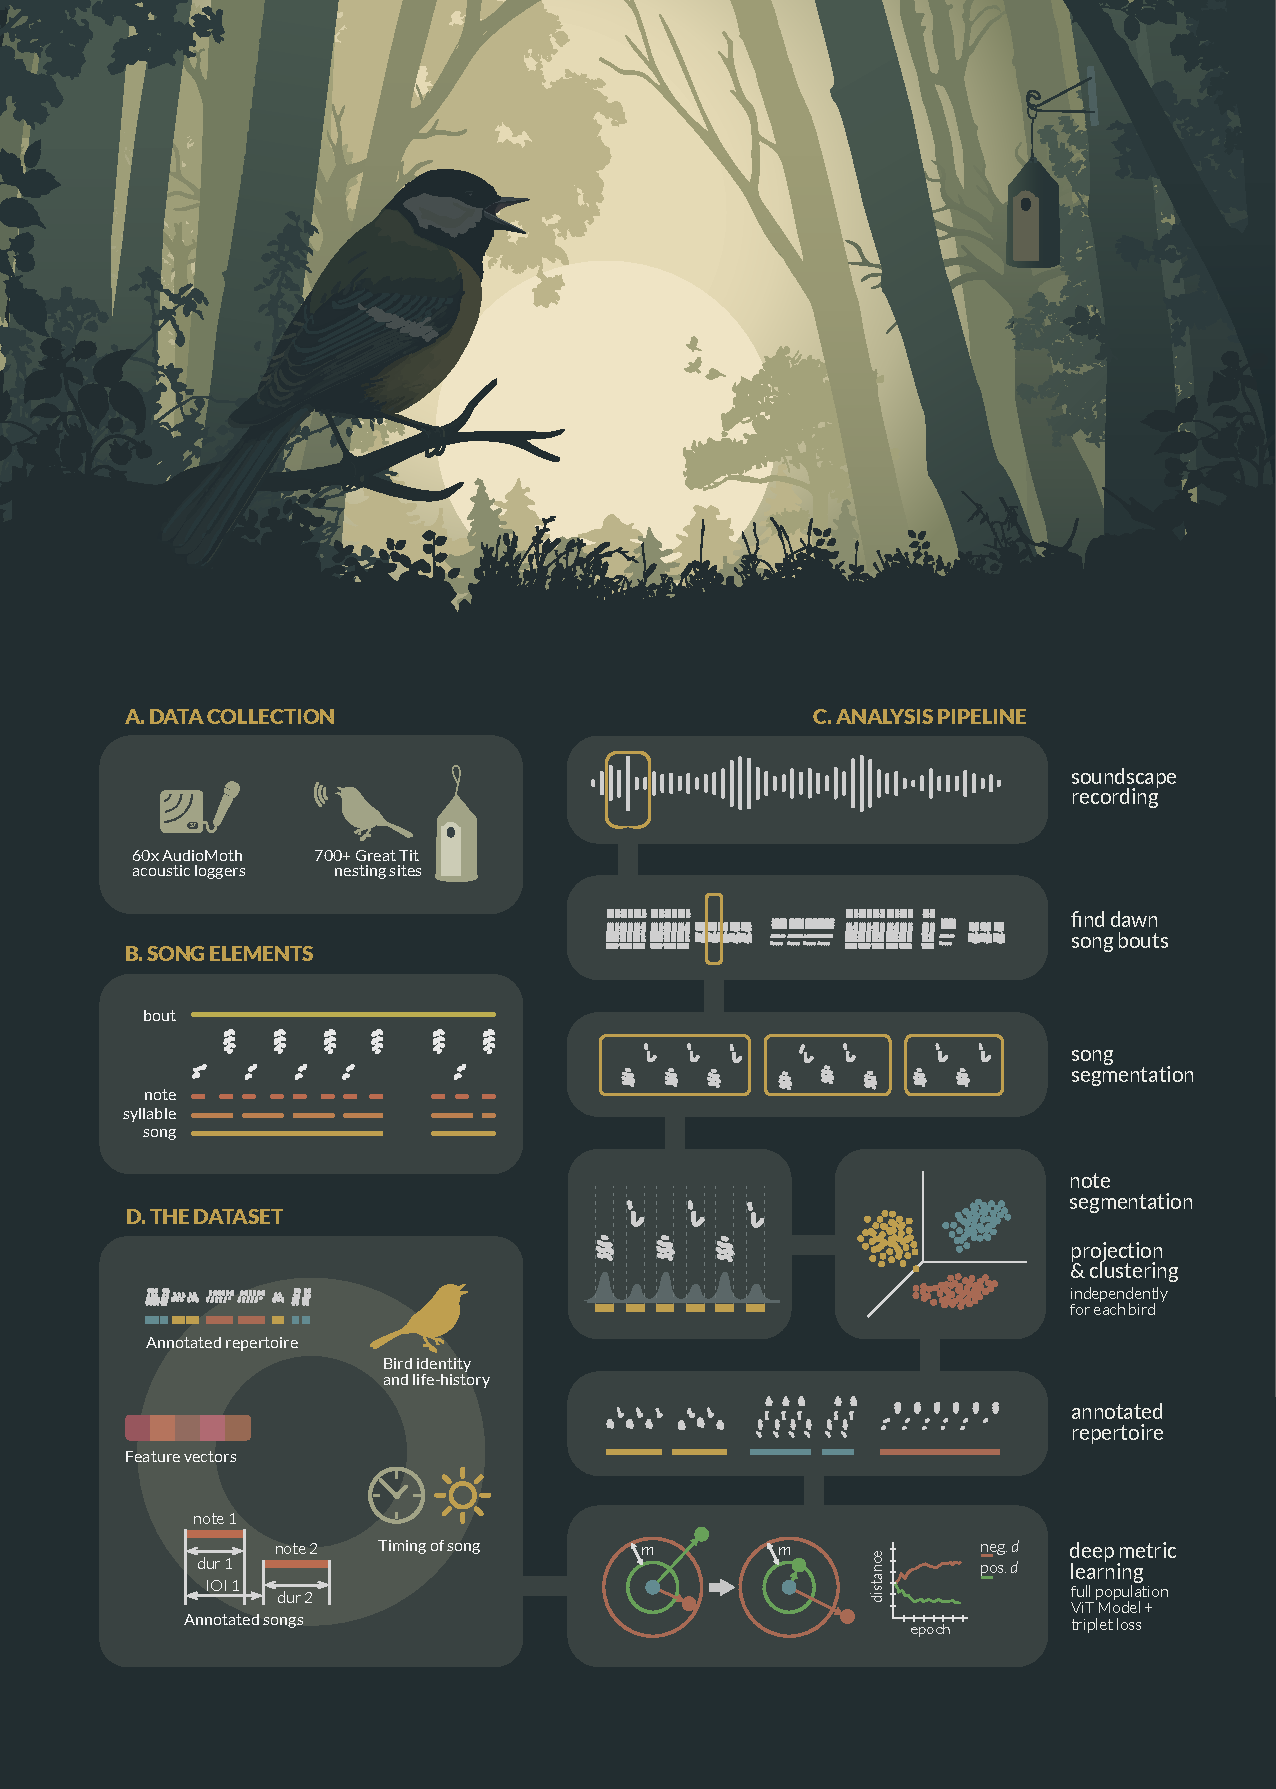
\includegraphics[width=\linewidth]{figures/chapter_3/FIG2-AB.pdf}
    \mycaption{Data collection and analysis pipeline used to prepare the Wytham great tit Song Dataset}{A brief visual summary of the data collection and analysis pipeline used to prepare the Wytham great tit Song Dataset. (A) Data collection in the field. (B) The terminology used to describe the various hierarchical levels at which we can describe great tit's singing. (C) Computational pipeline. (D) Main outputs included as part of the dataset.}
    \label{c3_fig:pipeline}
\end{figure*}
%%%%%

\subsection{Ethical note}
All work involving birds was subject to review by the University of Oxford, Department of Zoology, Animal Welfare and Ethical Review Board (approval number: APA/1/5/ZOO/NASPA/ Sheldon/TitBreedingEcology). Data collection adhered to local guidelines for the use of animals in research and all birds were caught, tagged, and ringed by BTO licence holders.

\subsection{Recording equipment and schedule}

We used 60 (30 in 2020) AudioMoth recorders \parencite{hill2019}, which were housed in waterproof, custom-built enclosures. Recording began approximately one hour before sunrise (05:36 -- 04:00 UTC during the recording period) and consisted of seven consecutive 60-minute-long recordings with a sample rate of 48 kHz, and a depth of 16-bit. To sample as many birds as possible, we left each recorder in the same location for at least three consecutive days before moving it to a different nest box. We relocated 20 recorders (10 in 2020) every day throughout the recording period.

% TODO: theis box causes errors, fix
\begin{tcolorbox}[colback=tablegrey, boxrule=0pt, colframe=white, sharp corners] %TODO: add label here
    \subsection{A note on terminology}
    There is no consistent terminology used to describe the various hierarchical levels of a bird's vocal production. For clarity, we adopt the terminology outlined in \cite{thompson1994}; see also \autoref{c3_fig:pipeline}B for a graphical explanation. 
    \medskip
    The fundamental temporal unit is referred to as a \textbf{note}. Notes are represented by continuous traces on the sound spectrogram and are separated by silences. Moving up the hierarchy, \textbf{syllables} are sequences of one or more notes that are always repeated in the same order. Beyond syllables, we have \textbf{songs}, which consist of clusters of the same type of syllables punctuated by longer pauses, often in the order of seconds. Lastly, song \textbf{bouts} are uninterrupted performances of songs of the same type. great tits tend to sing the same song type repeatedly before transitioning to a different type. They continue this pattern until they stop singing altogether, often after having performed their entire song repertoire.
\end{tcolorbox}

%%%%% FIG 3: QUERIES
\begin{figure*}
    \centering
    \includegraphics[width=\linewidth]{figures/chapter_3/FIG3-AB.pdf}
    \mycaption{A visual representation of the song spectrogram embedding space}{Measuring similarity is a very hard problem, in large part because there is often no objective way to compare the performance of different methods. Here, we took a data-based approach by training a Vision Transformer (ViT) model as a feature extractor in a Euclidean metric learning task. The resulting embedding space allows us to judge if two songs are very similar, and to re-identify birds. (\textbf{A}) PCA projection of the feature vectors: two orthogonal linear components do not capture much of the high-level distinguishing features. (\textbf{B}) This figure shows a UMAP projection of the 384-dimensional vectors for each song in the dataset into 2D, which leads to a fairly arbitrary but useful visualization where tight clusters of points correspond to song types in the repertoire of individual birds. They are coloured by how densely occupied that region of space is in the high-dimensional space, based on k=30 neighbours from other song types. (\textbf{C}) A k-nearest neighbour search returns the closest matches for a query vector (highlighted).}
    \label{c3_fig:queries}
\end{figure*}
%%%%%

\section{Data processing and annotation}

We processed and annotated the recordings using custom software and scripts written in Python 3 \parencite{vanrossum1995}, using the open-source package \texttt{pykanto} \parencite{merinorecalde2023}. These are available from \href{https://github.com/nilomr/great-tit-hits-setup}{\nolinkurl{github.com/nilomr/great-tit-hits-setup}} \parencite{nilo_gretidataset_setup_2023}. \hyperref[c3_fig:pipeline]{Figure \ref*{c3_fig:pipeline}} shows a graphic illustration of the process. See also Box 1 for a note on the terminology used for different parts of the songs.

\subsection{Song segmentation}

We inspected spectrograms for each raw recording and selected songs based on a simple criterion: that its notes were clearly distinct from background noise and other bird vocalizations. We chose entire songs where it was possible; where it was not, we selected the longest contiguous segment possible. This process was carried out manually using the open-source software Sonic Visualizer \parencite{cannam2010} by drawing boxes bounding songs in the time and frequency domains.

\subsection{Assigning song bouts to individuals}

Due to the automated recording process, there is a possibility that some of the recorded songs near a particular nest box may not originate from the focal bird. To minimize the chance of false positives, we discarded recordings with more than one vocalizing bird if one was not distinctly louder than the rest during the segmentation process. Additionally, we discarded all songs with a maximum amplitude below $-16$ dB, calculated as $20 \log_{10}\left(\frac{A}{A_0}\right)$, with $A = 5000$ and $A_0 = 32767$ (the maximum value for 16-bit digital audio). This specific threshold was derived from observations indicating that when simultaneous recordings captured neighbouring birds, an amplitude cut-off greater than 4000 consistently differentiated the focal bird from its closest neighbours. It is important to note that these are not calibrated values and are, therefore, relative to the recording equipment and settings we used --- as well as other factors like sound directionality and vegetation cover.

\subsection{Spectrogramming}

For most operations beyond this point, we used normalized, band-passed and log-scaled mel spectrogram representations of each of the songs (sampling rate = 22050,  window length = 1024, hop length = 128, mel bins = 224; see the repository \href{https://github.com/nilomr/great-tit-hits-setup}{nilomr/great-tit-hits-setup} for full details on the process).

\subsection{Note segmentation}

We segmented the resulting song selections into their constituent notes using a custom dynamic threshold algorithm implemented in pykanto \parencite{merinorecalde2023}, based on the work of \textcite{sainburg2019}. Briefly, the algorithm finds minima in the spectral envelope of a spectrogram, which are considered silences; if the length of the signal between these minima exceeds a maximum note duration, a new local minimum is defined that divides the signal into two shorter segments. This is repeated until multiple notes are defined or there are no local minima below a maximum amplitude threshold. Then, segments below a minimum note duration threshold are discarded. To make the algorithm more robust to noise, the spectrogram is subject to morphological transformations and de-echoing before amplitude information is extracted. The de-echoing algorithm implemented in pykanto is based on that in Luscinia \parencite{lachlan2016a}, and works by subtracting a delayed version of the spectrogram from itself. We determined minimum and maximum note length ranges by manually segmenting a small, random subset of songs (n = 30).

It should be noted that the automated segmentation process is susceptible to various factors that can influence its accuracy. These include background noise, significant variation in amplitude between notes, attenuation caused by vegetation, changes in the direction of sound production, and even variations in performance where some notes may be much quieter. As a result, the algorithm may fail to detect or incorrectly delimit certain notes. Despite this, we estimate that approximately 96\% of the notes are correctly segmented (0.037 error rate based on a random subset of n = 1048 notes that were checked manually). Still, depending on specific goals, we recommend manual verification of note segmentation if complete accuracy is crucial.

\subsection{Song type annotation}

We annotated each song type in the dataset using a semi-supervised approach implemented in \texttt{pykanto}. The process involved several steps to ensure accurate classification. First, we generated average unit spectrograms for each song by taking the mean of the centred and padded spectrograms of its units or notes, which provided a concise representation of the temporal and spectral characteristics of the syllable within it. Next, we performed non-linear dimensionality reduction using UMAP \parencite{mcinnes2018} and a cluster search using HDBSCAN \parencite{mcinnes2017} for each bird in the dataset. See \parencite{sainburg2020a, thomas2021} for similar approaches. This strategy, while useful, often leads to spurious outcomes. For instance, it may separate renditions of the same song type if variation in performance or background noise exists, or if certain song elements are sometimes attenuated. Such variation could be misinterpreted as distinct song types, leading to an overestimation of repertoire size. To address this, we used the interactive app in \texttt{pykanto} to review and split or combine clusters as necessary for each bird. It is worth mentioning that this process would be significantly more challenging in species with highly variable songs: our approach benefited from the great tits' relatively limited repertoires (1 to fewer than 15 song types in our population) and their tendency to produce stable and stereotyped songs.

\subsection{Calculating song embeddings}

Comparing animal vocalizations poses a significant challenge for researchers. Traditionally, two approaches have been used: visual comparisons of spectrograms and, more recently, measurement of hand-picked acoustic features \parencite{goffinet2021}. However, these methods have limitations when dealing with noise, variations in performance, and changes in syntax (where compositional syntax is not relevant). For instance, if a song with the sequence 'tea-cher, tea-cher' is recorded as 'cher-tea, cher', it might be wrongly perceived as highly dissimilar, despite being the same song (see \cite{stowell2021, zandberg2022} for a good overview of these issues). Additionally, these methods often fail to capture high-level features such as the syntactic relationships between notes and other complex spectrotemporal characteristics that cannot be easily characterized by an orthogonal combination of simple acoustic features.

\begin{table*}[ht!]
    \centering
    \mycaption{Short description of the files included in the dataset}{Short description of the files included in the dataset. See \href{https://nilomr.github.io/great-tit-hits}{the docs} for detailed documentation.}
    \label{table:summary}
    \begin{tblr}[
        theme=ntabs
        ]{
        colspec = {X[l]},
        rowsep=3pt,
        stretch = 0.8,
        row{odd} = {tablegrey}, % Shading for odd rows
        cells = {font = \fontsize{8pt}{8pt}\selectfont},
        row{1} = {font=\fontsize{8pt}{8pt}\selectfont} % First row is bold
    }
        109,963 raw song files with their corresponding metadata\\
        Model-based feature vectors, with 109,963 samples and 384 dimensions\\
        A main derived dataset including information on broods, adult bird life-history traits, nesting locations, and acoustic recordings\\
        Morphological measurements for birds captured and re-trapped in the study area. Includes information on species, age, sex, weight, and various other traits\\
        Information on the location and characteristics of nest boxes in Wytham Woods, along with a map of the site\\
    \end{tblr}
\end{table*}

Unfortunately, we cannot rely on the birds' perceptual judgements due to the lack of a hard to obtain experimental data (though recent studies, such as \cite{morfi2021, zandberg2022}, have explored this avenue). This can be an issue where the focus of research is behavioural interactions or the social functions of song. At the same time, for monitoring or individual identification purposes, fully mimicking the bird's perceptual space may not be ideal: the performance of metric learning or classification algorithms trained for narrow purposes can surpass the organism's abilities, as exemplified by facial recognition in humans \parencite{lu2014}. Here, our goal was to define a similarity space based on the inherent variation in the data and the only categorical labels that we know are perceptually and behaviourally significant: song types sung by individual birds. Given that great tits can recognize each other based on their vocalizations \parencite{lind1996}, we aimed to define a similarity space that facilitates similarity-based research and captures some of the song characteristics that birds themselves might attend to when distinguishing individuals. To do this, we took advantage of recent advances in the fields of deep learning and computer vision and used a data-driven approach. Below is a simple narrative description of the process. For further details, see the dedicated repository \href{https://github.com/nilomr/open-metric-learning/tree/great-tit}{nilomr/open-metric-learning} and the OML library \parencite{shabanov2023}. 


\subsubsection{Metric Learning and Vision Transformers}
Rather than focusing on classification, we aimed to develop semantically meaningful embeddings. To achieve this, we used a Vision Transformer (ViT) model as a feature extractor in a (Euclidean) metric learning task. These models, inspired by the success of transformers in natural language processing applications, process images by splitting them into patches, treating them as tokens similar to words in a natural language \parencite{dosovitskiy2021, raghu2022}. In this case, we used the ViT-S/16 architecture (21.7 M parameters), pre-trained on ImageNet using the DINO method (self-distillation with no labels; \cite{caron2021}), and fine-tuned of spectrogram representations of songs.

\subsubsection{Model Training}
During the training phase, we fine-tuned the ViT model using the great tit song dataset. To optimize the performance of the model, we used Triplet loss, a loss function that ensures that the projection of a positive sample, which belongs to the same class as the anchor point (i.e., song-type-within-individual), is closer to the anchor's projection than that of a negative sample, which belongs to a different class, by at least a specified margin \parencite{hermans2017, hoffer2018}. This loss function enables embedding points of the same class to form clusters without collapsing into a single point, which allows us to also explore differences within song types. While training the model we mined hard triplets---where the negative sample is closer to the anchor than the positive---and used the Adam optimizer with a fixed learning rate of $1 \times 10^{-5}$.

\subsubsection{Handling Data Imbalance and Batch Generation}
The distribution of song sample sizes per individual in the great tit dataset approximately follows a power law, resulting in a significant data imbalance. Although the use of triplet loss already addresses this issue to some extent \parencite{thakur2019}, we adopt a random subsampling strategy where classes with more than 100 samples are reduced to 100 for computational efficiency, classes with fewer than 15 samples are excluded to allow a large enough query/gallery split for validation, and we ensure fair representation during training using a balanced sampler \parencite{hermans2017}. Our batch generation strategy involves uniformly sampling P song types without replacement and sampling K spectrograms for each song type, with replication as necessary. This guarantees that all labels are selected at least once in each epoch.

\subsubsection{Train-Time Data Augmentation}
To enhance model robustness and prevent overfitting, we apply various train-time data augmentation techniques \parencite{mumuni2022, perez2017, shorten2019}. These include random cropping in the time domain, dropping out parts of the spectrogram, adding Gaussian and multiplicative noise, equalization, sharpening, changes to brightness and contrast, blurring, and slight shifting in both time and frequency domains. The latter augmentations are applied within the typical variation in performance observed in the great tit vocalizations.

\begin{table*}[ht!]
    \centering
    \mycaption{Description of the dataset and sample sizes}{A brief description of the dataset and sample sizes for different subsets of the data.}
    \label{table:samples}
    \renewcommand{\arraystretch}{0.8}
\begin{tblr}[
    theme=ntabs
    ]{
    colspec = {X[l] X[r]},
    rowsep=2pt,
    stretch = 0.8,
    row{odd} = {tablegrey}, % Shading for odd rows
    cells = {font = \fontsize{8pt}{8pt}\selectfont},
    row{1} = {tableheadgrey, font=\fontsize{8pt}{8pt}\selectfont\bfseries}, % First row is bold
}
    Description                                           & Value                \\
    Number of segmented notes                             & 1,161,033            \\
    Number of songs                                      & 109,963              \\
    Mean repertoire size                                 & 4.24                 \\
    SD repertoire size                                   & 1.98                 \\
    Median repertoire size                               & 4                    \\
    Number of unique classes                             & 1,930                \\
    Mean class size                                      & 56.98                \\
    SD class size                                        & 68.35                \\
    Median class size                                    & 31                   \\
    Number of nest sites recorded                        & 706                  \\
    Number of nest sites with data                       & 454                  \\
    Number of unique birds with data that were ID'd      & 242                  \\
    Number of times each bird was recorded               & 192 (1y), 42 (2y), 8 (3y) \\
\end{tblr}
\end{table*}

\subsubsection{Results}
Our trained model shows very good performance, achieving a mean Average Precision at 5 (mAP\@5) of 0.98 and a Cumulative Matching Characteristic at 1 (CMC\@1) of 0.98. This indicates that in approximately 98\% of the queries made to the similarity space, the returned candidate song type by a bird is the correct one. Errors primarily stemmed from instances where songs of the same type sung by the same bird appeared more than once in the dataset, which happened if a bird survived to the next year. Given that the model was trained on almost 2000 classes, this means that there is enough individual information contained in each song type to distinguish between birds with high confidence, which has important implications for both the study of individuality and population monitoring. See \hyperref[c3_fig:queries]{Figure \ref*{c3_fig:queries}} for a visual representation of the embedding space and nearest-neighbour queries.

\section{Data records and description}

\hyperref[table:summary]{Table A\ref*{table:summary}} contains a summary of the files included with the dataset. Detailed data documentation, including variable descriptions, can be found online at \href{https://nilomr.github.io/great-tit-hits/}{nilomr.github.io/great-tit-hits}.

The dataset provides a comprehensive view of the populations' natural dawn singing behaviour over three spring seasons. It documents changes in individual performance, the appearance and disappearance of birds---and with them, their songs---and highlights just how much behavioural variation there is along every dimension of what could at first seem a relatively simple trait. \hyperref[table:samples]{Table \ref*{table:samples}} presents some simple summary statistics, and \hyperref[c3_fig:summary]{Figure \ref*{c3_fig:summary}} provides a visual overview of the dataset.

Even though most birds in the dataset are one or two-year-olds recorded within a single year (which can be attributed to high turnover rates in the population given low annual survival), the dataset includes valuable data on much older individuals, including a 7-year-old. Among the recorded birds, some display metronome-like regularity in their performance, while others have highly variable or unusual songs, due to learning from allospecific vocalizations, or even issues with their vocal apparatus. You can find some interactive examples at \href{https://nilomr.github.io/great-tit-hits/}{nilomr.github.io/great-tit-hits}. The longest song recorded is approximately 20 times longer than the shortest song (and, coincidentally, was sung by one of the largest great tits ever recorded in the Wytham population). The median number of songs per song type and per bird in the dataset is 31, with a significant number of birds having a much larger count, reaching into the thousands; the median repertoire size per bird is four song types, although some birds performed as many as 13 distinct song types.

\subsection{Known biases and problems}

Working with third-party datasets can be challenging, perhaps particularly so in the study of behaviour in natural populations. The familiarity that fieldworkers inevitably develop with the study system and the data is difficult to replace, and, as a result, there is a risk of unintentionally overlooking important sources of bias and variability. We have compiled a list of some key considerations, which, while not exhaustive, can serve as a starting point for identifying and addressing biases when testing hypotheses, estimating parameters, or evaluating findings from the data. These issues can be broadly classified into two groups: those around bird and song type labelling, which can be partially addressed, and those that are inherent in the data or how it was collected.


\subsubsection{Individual and song identification}

One factor that can be partially addressed is that the birds recorded in our dataset are not a random subset of the population; they are those that establish territories and begin the breeding process. In turn, birds that are subsequently identified are more likely to be those whose chicks hatch and survive for at least six days, when the first identification attempt is made. This may skew the distribution of certain behaviours within the dataset or lead to endogenous selection bias \parencite{elwert2014}. One way to quantify the extent to which the subset of identified birds is representative of the entire breeding population would be to compare the distribution of the trait of interest in both groups. See, for example, \cite{kidd2015}, who found that females in nests that fail early in our population are more likely to be immigrant birds breeding in poor-quality areas.

Another issue to consider is that birds may attempt to breed again in the same nest box or elsewhere after a failed attempt. This, coupled with a failure to identify the male associated with those attempts, means that it is conceivable (although likely very rare) that songs from the same bird could appear in the same year twice, leading to pseudoreplication. Similarly, unidentified birds present in the dataset for multiple years could contribute to this problem. One potential way to address these issues is by using song embeddings for identification based on similarity and assigning dummy IDs to birds believed to be the same individual. At least, this should be modelled to assess the sensitivity of any results to varying degrees of pseudoreplication from this source.

Finally, a few songs might have been mislabelled before model training, as it is not feasible to manually check such a large dataset. However, the model-based embeddings can help identify any mislabelled songs: they will be clear outliers within their respective classes, thanks to the relatively discrete nature of great tit repertoires.


\subsubsection{Unequal samples; songs and calls---and female song}

As is common in many complex systems, the interaction of the many processes involved in both song production and sampling results in a heavy-tailed frequency distribution of sample sizes. This variation stems from various sources, including characteristics inherent to the study system, such as individual differences in singing activity and temporal fluctuations throughout spring. The sampling process introduces further variation, through factors like equipment malfunctions causing small gaps in the data, variation in recording dates relative to peak activity, and the impact of rain and hail on singing activity and recording quality. We cannot assume these processes to be completely independent of each other. Therefore, when analysing song output or repertoire size, it is important to explicitly specify the assumed causal relationship between factors such as individual characteristics, sampling probability, and the outcome measure.

Another important aspect to consider is that, while we have said that the dataset consists of songs, the demarcation between songs and calls is not entirely straightforward. Some vocalizations that would typically be classified as calls, due to their acoustically simpler, shorter, and possibly more stereotyped nature, are actually used as part of the dawn vocal behaviour. These vocalizations are repeated in a manner that creates an impression of functional equivalence to songs. While we have followed criteria similar to other studies \parencite{baker1986, fayet2014, krebs1978, rivera-gutierrez2010a} to maintain consistency, we believe that this phenomenon warrants further attention. These calls were not segmented and thus are not included in the dataset, but we are happy to provide soundscape recordings to anyone interested in exploring this aspect further.

Finally, although female song in birds has received relatively little historical attention (see \cite{langmore2020, odom2018, riebel2005} for further discussion), female great tits also sing (see a brief treatment in \cite{gompertz1961, hinde1952}). The vast majority of songs in the dataset belong to the dawn song, a behaviour exclusively performed by the male prior to the female leaving the nest (a pattern observed in blue tits as well, as documented by \cite{sierro2022}). Females, on the other hand, vocalize within the nest, but these vocalizations \parencite{gorissen2005, gorissen2004} differ from songs and were not typically detectable by our recording devices. Nevertheless, \cite{hinde1952} suggests that in the absence of males, females may be more inclined to engage in territorial behaviour that involves singing rather than just producing calls. If that is the case, it is possible that our dataset contains some isolated instances of female song.

%%%%% FIG 4: 
\begin{figure*}[th!]
    \centering
    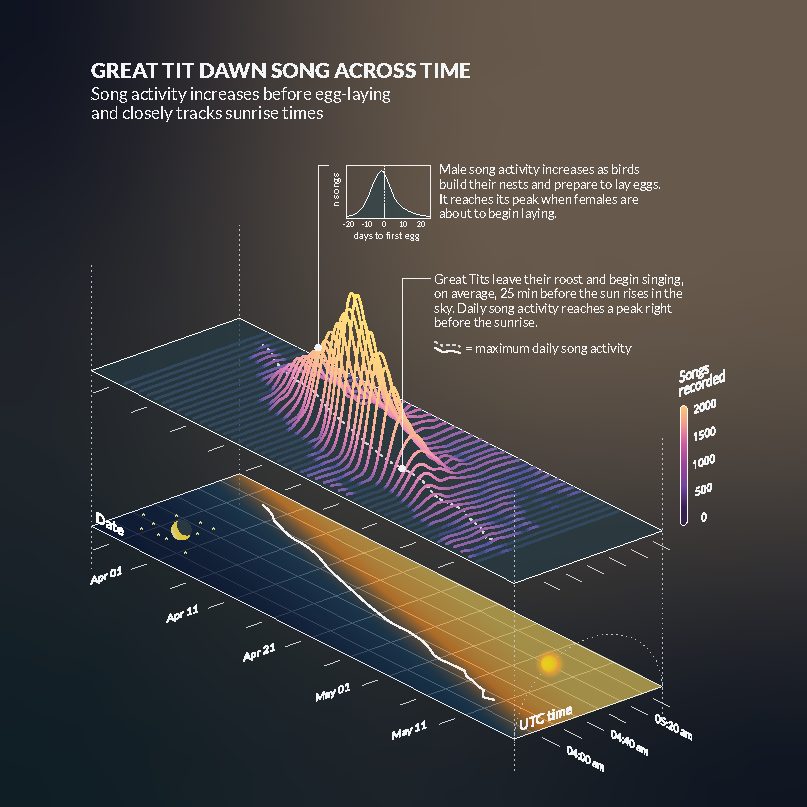
\includegraphics[width=\linewidth]{figures/chapter_3/FIG4-AB.pdf}
    \mycaption{Great tit song activity closely tracks advancing sunrise times and female fertility}{Days get longer as the spring progresses and male great tits track the advancing sunrise times with great precision, so that they always begin singing, on average, 25 minutes before the morning breaks. This figure also shows (z-axis) how song activity peaks alongside egg laying: males sing the most in the morning right before their partner lays the first egg.}
    \label{c3_fig:timing}
\end{figure*}
%%%%%

\section{Uses and suggestions}

The dataset we are presenting contains detailed information about the vocal behaviour and life of wild birds, providing valuable opportunities for investigating a wide range of research questions. In this section, we suggest several research areas that can be explored using this dataset and provide references to relevant studies in the literature.

\textbf{Behavioural repeatability and stability across multiple scales}: Researchers can use the dataset to examine the repeatability and stability of song production and song characteristics across different temporal and spatial scales. This includes studying consistency in vocal behaviour within individuals over time and across different contexts, and its links to age \parencite{rivera-gutierrez2012, zipple2019} and reproductive fitness \parencite{sierro2023}.

\textbf{Links between vocal performance or diversity and reproductive success}: Our data can be used to explore the relationships between vocal performance metrics, such as song complexity or vocal diversity, and individual breeding success on a dataset that is much larger than what is typical in the field \parencite{hutfluss2022, beecher2020a, crates2021, hiebert1989, mcgregor1981}. 

\textbf{Spatial and temporal properties of acoustic communities}: The dataset enables investigations into the spatial properties of acoustic communities, including the distribution of singing individuals within a given habitat and across time. This can provide valuable insights into the spatial dynamics of communication networks and acoustic interaction among neighbour birds.

\textbf{Timing and volume of song production}: Researchers can use the dataset to analyse the temporal patterns and timing of song production in great tits. This might involve studying diurnal variation, seasonal trends, and the influence of environmental factors on the timing and abundance of vocal behaviour. As an example, \hyperref[c3_fig:timing]{Figure \ref*{c3_fig:timing}} provides an overview of key temporal shifts in dawn singing behaviour: male birds sing more during the fertile period of the female, and their activity closely tracks advancing sunrise times.

\textbf{The syntactic organization of song production}: The dataset captures song activity over entire dawn song periods, across days, and even years for many individuals. This would allow researchers to investigate the set of rules that govern the arrangement of song elements and transitions within the vocal repertoire of wild great tits, in terms of short and long-distance dependencies and other properties of their sequential dynamics \parencite{hedley2018, lachlan2010, sainburg2019, searcy2022}.

\textbf{Song learning in the wild}: While this dataset does not directly provide evidence of song learning, researchers can use song similarity and proximity in time and space to infer cultural transmission processes. This allows for the exploration of the influence of spatial and social factors on song learning \parencite{james2020, lachlan2003, nelson2014, peters2017, wheelwright2008}.


\section{Conclusion}

With over 1,100,000 annotated notes and acoustic units from more than 100,000 songs, collected over three spring seasons, we hope that this dataset will offer valuable insights into bird vocal behaviour and song culture. The dataset is enriched with detailed metadata such as note onset and offset times, song type labels and embeddings derived from a deep metric learning model, as well as identity and life-history information for the birds, which makes it useful for a wide range of research purposes. By sharing this comprehensive dataset, we also aim to help promote data-sharing and scientific collaboration.

\section{Author contributions}

LP, AV, AE and NMR collected the data. NMR created the software and pipeline to plan fieldwork and analyse the data, annotated the dataset with help from AE, built the website, documentation, and visualizations, and wrote the original draft. BCS and EFC provided feedback and supervision throughout the research, and all authors contributed critically to drafts.

\section{Acknowledgements}
We thank all those who have contributed to the long-term nest box study in Wytham Woods and the collection of associated data.
This work was supported by a Clarendon-Mary Frances Wagley Graduate Scholarship
and an Edward Grey Institute scholarship to Nilo Merino Recalde and made use of the University of Oxford Advanced Research Computing facility \parencite{richards2015}.

\section{Conflict of interest statement}
The authors declare no conflict of interest.

\section{Data and code: availability and use}

The complete Wytham great tit Song Dataset and its metadata are available at \href{https://osf.io/n8ac9/}{\nolinkurl{10.17605/OSF.IO/N8AC9}} \parencite{nilo_gretidataset_osf_2023}. The code to train the deep metric learning model can be found at \href{https://github.com/nilomr/open-metric-learning/tree/great-tit}{nilomr/open-metric-learning}. See the \href{https://nilomr.github.io/great-tit-hits/}{dataset website} for documentation and more information.

All input and output data files use open data formats and are under a \href{https://creativecommons.org/licenses/by/4.0/}{CC-BY-4.0} licence. The scripts and software used to create this dataset are available under the \href{https://github.com/nilomr/pykanto-example/blob/main/LICENSE}{MIT} licence from GitHub \href{https://github.com/nilomr/great-tit-hits-setup}{nilomr/great-tit-hits-setup} and archived at Zenodo \parencite{nilo_gretidataset_setup_2023}.

\renewcommand{\cleardoublepage}{}
\renewcommand{\clearpage}{}
\printbibliography

    \end{multicols} % end one-column layout
    \onecolumn




% % % Chapter 4: The demographic drivers of change in wild bird song culture: ==============

\runningauthor{Merino Recalde \textit{et al}., 2023}
\fancyhead[LE]{\sffamily\color{black50}\thepage\hspace{2em}The demographic drivers of change in wild bird song cultures}
%\runningtitle{The demographic drivers of change in wild bird song cultures}
\clearpage{\pagestyle{empty}\cleardoublepage} % empty page before chapter
\onecolumn % start one-column layout for chatper 4

    \chapter{The demographic drivers of change in wild bird song culture: an individual-based study}
    \vspace{10pt}
    \thispagestyle{empty}  % remove page number 
    {\normalfont\sffamily\raggedleft
    {Nilo Merino Recalde \orcidlink{0000-0003-3903-1288}\textsuperscript{1,$\ast$}, 
    Andrea Estandía \orcidlink{0000-0002-3895-2141} \textsuperscript{1}, 
    Ella F. Cole \orcidlink{0000-0002-2689-946X}\textsuperscript{1}, 
    and Ben C. Sheldon \orcidlink{0000-0002-5240-7828}\textsuperscript{1}\par
    \vskip 0.7em

    {\small\textsuperscript{1}Edward Grey Institute, Department of Biology, University of Oxford, Oxford, UK\par}
    \small\textsuperscript{$\ast$}Corresponding author: \href{mailto:nilo.recalde@biology.ox.ac.uk}{nilo.recalde@biology.ox.ac.uk}

    } }

    \mysummary{
        \noindent Social learning within communities sometimes leads to behavioural patterns that persist over time, which we know as culture. Examples of culture include learned bird and whale songs, cetacean feeding techniques, and avian and mammalian migratory routes. Shaped by neutral and selective forces, animal cultures evolve dynamically and lead to cultural traditions that differ greatly in their diversity and stability. These cultural traits can influence individual and group survival, population structure, and even inform conservation efforts, underscoring the importance of understanding how other population processes interact with social learning to shape culture. Although the impact of social learning biases and mechanisms has been extensively explored, the role of demographic factors---such as population turnover, immigration, and age structure---on cultural traits has received theoretical attention but rarely empirical investigation in natural populations. Doing so requires very complete trait sampling and detailed individual life history data, which are hard to acquire in combination. To this end, we built a multigenerational dataset containing over 109,000 songs from >400 individuals from a population of Great Birds (\textit{Parus major}), which we study using a deep metric learning model to reidentify individuals and quantify song similarity. Our findings highlight that demographic variation at the small spatial scales at which learning takes place has the potential to strongly impact the pace and outcome of animal cultural evolution. For example, age distributions skewed towards older individuals are associated with slower cultural change and increased diversity, while higher local population turnover leads to elevated rates of cultural change. Our analyses support theoretical expectations for a key role of demographic processes resulting from individual behaviour in determining cultural evolution, and emphasise that these processes interact with species-specific factors such as the timing of song acquisition. Implications extend to large-scale cultural dynamics and the formation of dialects or traditions.}

    {\small\textsf{\textbf{Keywords:} animal culture; bird song; demography, cultural evolution}}

    \vspace{.5cm}

% Begin chapter proper
\begin{multicols}{2} % start one-column layout
\section{Results and Discussion}

Some behavioural traits are shared and persist within communities due to social learning \parencite{viciana2021}. We refer to these behaviours as 'animal culture', exemplified by tool use in capuchin monkeys \parencite{falotico2019}, the learned songs of oscine birds, migration routes \parencite{jesmer2018, berdahl2018, byholm2022}, and the feeding techniques of some cetaceans \parencite{allen2013, rendell2001}. Animal cultures are not static: neutral and selective mechanisms influence the frequency of cultural traits \parencite{potvin2015, williams2021}, leading to a process of cultural evolution. The resulting cultural traditions vastly differ in their diversity and stability \parencite{tchernichovski2017}, determined by both learning biases and mechanisms and the demographic structure of populations \parencite{deffner2022a, kandler2017}. 

While the role of social learning strategies and biases---frequency dependence, tutor biases, etc.---has been extensively studied \parencite{pike2010, kendal2015, aplin2017, lachlan2018, tchernichovski2021}, there exists a substantial gap in our understanding of how demography contributes to the emergence and persistence of distinct cultural traits within wild populations. Processes such as the recruitment of juveniles and immigrants, emigration, mortality, and variation in age structure are likely to strongly affect an individual's opportunities for learning and exposure to different cultural variants, which has been amply emphasised by theoretical work \parencite{deffner2022a, deffner2022, kandler2023, fogarty2019, deffner2020, derex2016, kirby2021, nunn2009, barta2023}. Despite this, translating theoretical expectations into empirical evidence remains a challenge. (See \cite{chimento2021, fayet2014} for exceptions). 


\begin{figure*}[hbt!]
    \centering
    \includegraphics[width=\linewidth]{figures/chapter_4/FIG1.pdf}
    \mycaption{Study system and main variables in our analysis}{
        (A) Cultural variables measured at the neighbourhood level. See methods for definitions.
        (B) Variation in the properties and composition of neighbourhoods across the population. See methods for definitions.
        (C) 3D render of our study site, Wytham Woods, based on first return LiDAR data \parencite{defra2020}. Elevation is exaggerated. The network represents pairwise song cultural distances between individuals with known spatial locations, used in the models reported in Fig. 2. Aquamarine (darker) arrows represent natal dispersal within the population, and the yellow (lighter) arrow represents immigration into the population, two of the variables used in this work. Age and bird (individual) turnover are not depicted.        
    }
    \label{c4_fig:main}
\end{figure*}


Culture is increasingly recognised as both a fundamental aspect of many animals' lives and a valuable tool in monitoring and conservation efforts \parencite{brakes2019, brakes2021}: cultural traits play a role in the survival and reproduction of individuals and social groups; they reflect or even shape the structure of the population \parencite{brakes2019}, and can be lost when habitat fragmentation and population decline lead to reduced learning opportunities \parencite{paxton2019, crates2021}. A comprehensive understanding of cultural change and loss, then, requires that we have the ability to detect and study not just intrinsic factors---social, cultural, cognitive---but also extrinsic, ecological and demographic processes. This entails identifying the relevant spatial and temporal scales at which these processes manifest within natural populations, as well as their relative importance.


\begin{figure*}[th!]
    \centering
    \includegraphics[width=\linewidth]{figures/chapter_4/FIG3.pdf}
    \mycaption{Influence of demographic variables on cultural diversity and novelty}{
        (A) Marginal effects at the mean of neighbourhood characteristics including mean dispersal distance, proportion of immigrant birds, average age, and individual turnover.
        (B) Adjusted predictions and partial residuals of the effect of mean dispersal distance on cultural novelty. Low-dispersal neighbourhoods are those in which birds were born in the same area.
        (C) Adjusted predictions and partial residuals of the effect of the mean age of the neighbourhood on cultural diversity. A neighbourhood with a mean age of 1 would be one where all birds are breeding for the first time.
        (D) The average distribution of cultural diversity in the population across space during the study period (2020-2022). This map captures the residual variation in cultural diversity after taking into account the demographic variables in (A). The map is based on a Gaussian process model with a exponentiated-quadratic kernel covariance function, which allows us to interpolate between the locations where we have data.
    }
    \label{c4_fig:diversity}
\end{figure*}


To contribute to this goal, we built a comprehensive dataset that spans three years and documents the dawn songs produced by male Great Tit birds during 454 breeding attempts in a single population located in Wytham Woods, UK. This population has marked variation in individual turnover, postnatal dispersal distances, age structure, and immigration across space (\autoref{c4_fig:main}), which allowed us to estimate their effects on song cultural repertoires at both individual and group levels within the long-term population study of this species \parencite{lack1964}. First, we assign more than 109,000 songs in 330 song repertoires to 242 individual birds through a combination of direct physical capture, radio frequency identification microchips, and a novel song-based reidentification method using a deep metric learning model. Then we quantified individual and group-level traits and analysed variation in song cultural similarity, diversity, and turnover using network and spatial Bayesian multilevel regression models.

Our results reveal an interplay of demographics and song culture dynamics that, albeit complex, largely matches theoretical expectations, as discussed below. This work also demonstrates that bird song, which already provides what is perhaps the largest body of evidence for cultural change in animals \parencite{laland2006}, also has the potential to help us shed light on the impact of other population processes, thanks to the fact that we can sample song cultural repertoires with relative ease.


\subsection{Reduced dispersal, increased immigration and an aged population are associated with higher cultural diversity}

Population genetics provides robust evidence supporting the notion that high dispersal rates facilitate gene flow, which, in turn, reduces the efficacy of selection and diversification. Conversely, low dispersal facilitates genetic differentiation through mechanisms such as mutation and drift, leading to allopatric population divergence \parencite{suarez2022, claramunt2011, papadopoulou2009}. Drawing an analogy from genetics to culture, we anticipate that reduced dispersal rates would decelerate the diffusion of cultural traits \parencite{nunn2009}. This, in turn, would result in the maintenance of distinct behavioural patterns within populations \parencite{whitehead2012, planque2014}, leading to a greater abundance of cultural variants unique to a specific area. Our analysis indeed indicates that neighbourhoods where more birds have remained in close proximity to their natal areas harbour greater cultural diversity and novelty (\textit{diversity:} $P(\beta_{disp (\overline{m})} < 0 | D) = 1,~ mem = -0.018,~CI_{95\%}~[-0.023, -0.012]$; \textit{novelty:} $P(\beta_{disp (\overline{m})} < 0 | D) = 0.96,~ mem = -0.005,~CI_{95\%}~[-0.01, 0]$; \figref[a\&b]{c4_fig:diversity}, \autoref{table:model_estimates}), in line with prior research at a coarser grain \parencite{fayet2014}. 

However, the analogy breaks down when we examine our individual-level models more closely. Although the outcome at the group level resembles the homogenization of populations resulting from gene flow, the underlying mechanisms differ significantly, due to a complex interaction of the timing of dispersal and learning mechanisms that are species-specific. In the case of Great Tits, these mechanisms are believed to involve selective retention or modification of songs encountered during early life and dispersal, a process that results in crystallized song repertoires that closely resemble those of their new neighbours at breeding sites \parencite{marler1982, peters2017, nelson1992}. Birds that dispersed over longer distances tend to have repertoires composed of songs that are common within the population (\textit{novelty:} $P(\beta_{disp (m)} < 0 | D) = 1,~mem = -0.2,~CI_{95\%}~[-0.3, -0.09]$; \figref[b]{c4_fig:individual}, \autoref{table:model_estimates}), and possibly smaller repertoires as well (\textit{rep.size:} $P(\beta_{disp (m)} < 0 | D) = 0.91,~mem = -0.2,~CI_{95\%}~[-0.44, 0.05]$; \figref[b]{c4_fig:individual}; \autoref{table:model_estimates}). We speculate that birds with more extensive movements are, on average, more likely to sample cultural variants that are common across the population. In contrast, birds with a more restricted and stable neighbour pool tend to be equally exposed to common and globally rarer songs, and this is enough to give rise to the differences that we estimate at the group level.



\begin{figure*}[]
    \centering
    \includegraphics[width=\linewidth]{figures/chapter_4/FIG2.pdf}
    \mycaption{Individual and dyadic analysis of cultural diversity and similarity}{
        (A) Illustrative example showing the repertoires of two different birds in the population, with three songs in each, one of which is shared. Each subpanel shows a stylised spectrogram, with time in the horizontal axis and frequency in the vertical. Units not shown.
        (C) Marginal effects (ME) of dispersal, immigration status, and age on song repertoire similarity between individuals. Dispersal: Birds that are close neighbours are more culturally similar, regardless of where they were born, whereas natal distance may have a weak positive effect on cultural similarity. Immigration: There is no strong evidence that birds born outside the population are dissimilar from resident birds. Age difference: Birds are less culturally similar the greater the difference in their birth years.
    }
    \label{c4_fig:individual}
\end{figure*}

Building on our understanding of cultural dynamics in relation to dispersal we expect that, when song learning is relatively precise and dispersal is limited, cultural differences will accumulate, and long-distance dispersal events will introduce cultural novelty to the recipient population. However, the extent to which immigration introduces new cultural variants into the population also hinges on an interplay between the species' learning programme, the timing of dispersal, and the spatial movements of individuals. Animals that learn first and then disperse, for example, may bring cultural novelty with them. But this is not the case for Great Tits, whose young disperse in late summer and autumn, shortly after achieving independence; learn their songs until the end of their first winter \parencite{rivera-gutierrez2011}, and become chiefly sedentary as adults \parencite{greenwood1979, dhondt1979, dingemanse2003}. In this species, then, we anticipate that immigrant birds will learn or retain songs they encounter upon arrival, either before or during the establishment of their territories \parencite{keen2020, graham2018}. 

Indeed, in our study, we find no evidence that the repertoires of birds originating from outside the population significantly differ from those of resident birds ($mem = -0.002,~CI_{95\%}~[-0.006, 0.002]$; \figref[c]{c4_fig:individual}). This, in conjunction with the observation that cultural similarity between individuals is predicted by the distance between breeding territories ($mem = -0.005,~CI_{95\%}~[-0.006, -0.004]$; \figref[c]{c4_fig:individual}; \autoref{table:model_estimates}), supports the hypothesis that Great Tits are predominantly closed-end learners that learn primarily from territorial neighbours after dispersal \parencite{mcgregor1982b, rivera-gutierrez2011, graham2017}.

This leads to a somewhat contradictory scenario, however: immigrant birds, while not acoustically distinct, tend to exhibit larger repertoires compared to their resident counterparts (\figref[b]{c4_fig:individual}; $P(\beta_{\overline{imm}.} > 0 | D) = 0.87,~mem=0.24,~CI_{95\%}~[-0.098, 0.593]$; \autoref{table:model_estimates}). At the group level, this small and uncertain effect amplifies, such that neighbourhoods with a higher proportion of immigrant birds do not exhibit increased cultural diversity relative to the total number of songs ($mem=~0.002~CI_{95\%}~[-0.004, 0.007]$; \figref[a]{c4_fig:diversity})---but they do have a higher absolute cultural diversity---above what would be expected based solely on the number of birds ($P(\beta_{\overline{imm}.} > 0 | D) = 0.98,~mem=0.47,~CI_{95\%}~[0.1, 0.84]$; \autoref{fig:supp_absolute_cultural_diversity}, \autoref{table:model_estimates}). 

Previous research \parencite{verhulst1997} has revealed that most birds arriving from outside the population disperse over two kilometres, significantly farther than the typical distances observed within the population (median for males = 558 metres \parencite{greenwood1979}). This extended dispersal may have qualitative effects on the process, through a combination of factors: first, an initial exposure to songs from the source population; then, a heightened pressure to adopt vocalizations similar to those of territorial neighbors to avoid any social or reproductive costs associated with non-local signals \parencite{payne1983, baker1981, mortega2014, lachlan2014, beecher2008}.

Finally, we find that individual turnover does not significantly affect cultural diversity or novelty, and we uncover an association between age structure and cultural diversity and novelty (\figref[b]{c4_fig:diversity}). Individuals of the same generation share the most similar song repertoires and, while age itself doesn't directly relate to changes in the repertoires of individual birds (\figref[b]{c4_fig:individual}), the acoustic similarity between any pair of individuals decreases as the age gap between them widens (\figref[c]{c4_fig:individual}; \autoref{table:model_estimates}). This is expected when a species ceases to learn new songs as they age, and it has detectable consequences for neighbourhoods: those with a higher proportion of old individuals have heightened levels of cultural diversity and novelty. Conversely, in areas where the majority of the population comprises active learners surrounded by their peers, birds tend to produce fewer unique songs that are simultaneously more typical (\figref[a]{c4_fig:diversity}; \autoref{fig:supp_absolute_cultural_diversity}; \textit{diversity:} $P(\beta_{\overline{age}} < 0 | D) = 1,~mem=0.021,~CI_{95\%}~[0.014, 0.027]$; \textit{novelty:} $P(\beta_{\overline{age}} < 0 | D) = 0.99,~mem=0.012,~CI_{95\%}~[0.005, 0.019]$).

\begin{figure*}[th]
    \centering
    \includegraphics[width=\linewidth]{figures/chapter_4/FIG4.pdf}
    \mycaption{Influence of demographic variables on the rate of local cultural change}{
        (A) Marginal effect at the means for mean dispersal distance, proportion of immigrant birds, average age, and individual turnover on the rate of cultural turnover.
        (B and C) Adjusted predictions and partial residuals of the effects of the proportion of individual turnover on cultural turnover (B) and the effect of mean neighbourhood age on cultural turnover (C).
        (D) The population's average distribution of cultural turnover across space during the study period (2020-2022).
        (E) Posterior counterfactual predictions for two scenarios: all variables at their maximum (Max.) and minimum (Min.) observed values, adjusting for individual turnover. Cultural turnover is expected to be over two times higher when neighbourhood dispersal, immigration and age are low.
    }
    \label{c4_fig:turnover}
\end{figure*}

\subsection{Demographic processes strongly moderate the rate of cultural change at small spatiotemporal scales}

We now shift our focus from static measures of cultural diversity to cultural turnover, examining how quickly song variants disappear from neighbourhoods and the consequences this has for their cultural makeup. The primary driver of cultural turnover is individual turnover (\textbf{total effect} $mem = 0.072~CI_{95\%}~[0.051, 0.093]$): as birds leave or die, many song variants go with them. Accounting for this, we also assess the direct impact of average natal dispersal distance, the proportion of immigrant birds, and average neighbourhood age: higher levels of each of these factors correlate with slower cultural change in the neighbourhood (\figref[a]{c4_fig:turnover}; \autoref{table:model_estimates}). When there is substantial dispersal, a high influx of immigrants, and an age distribution skewed towards older individuals, the model predicts slower cultural change, at less than half the rate compared to the converse scenario ($0.28~CI_{95\%}~[0.23, 0.34]$ vs. $0.61~CI_{95\%}~[0.49, 0.76]$, as illustrated in \figref[e]{c4_fig:turnover}).
Modelling work suggests that learning from older individuals should slow down cultural change \parencite{kirby2021}, aligning with our observations ($P(\beta_{\overline{age}} < 0 | D) = 1,~mem=-0.044,~CI_{95\%}~[-0.063, -0.026]$; \figref[c]{c4_fig:turnover}). Age may serve as a brake on change, potentially increasing the relative cultural diversity and novelty within neighbourhoods compared to the broader population by maintaining song types now less frequent in the population, as supported by the individual-level analysis where birds become more dissimilar as they are further in time.
Across the three-year study period, now considering the entire population, cultural turnover between consecutive years hovers around 45\% (0.47, 0.44). If all variants faced an equal chance of disappearing, this high turnover rate would lead to complete cultural replacement within a short time span. However, with a two-year gap, turnover only slightly increases to 0.59. We expect this rate to taper over longer periods, as rare variants encounter greater stochasticity while common songs endure (\figref[a]{fig:supp_song_frequencies}. This is exemplified by some common song types documented over four decades ago that persist within the same population \parencite{mcgregor1982b, keen2020}, either through accurate learning or, more likely, strong convergent biases \parencite{lachlan2018, tchernichovski2021, james2017, claidiere2007}.


\subsection{Consequences for cultural structure, stability and diversity}

Cultural traits, learnt bird song in this case, are shaped by many different factors: some external, such as those discussed here, others intrinsic to learning and culture, and yet others driven by selective processes driven by preference and function. Even within the confines of a relatively small population---Wytham Wood spans a mere four kilometres---we have recovered associations between heterogeneity in the demographic composition of neighbourhoods and cultural outcomes, which emphasises the need for both empirical studies and modelling efforts on cultural change to account for the population's demographic characteristics and their inherent heterogeneity across time and space, which shape individuals’ exposure to cultural variants and opportunities for learning and, therefore, emergent group-level cultural dynamics.

\section{Methods}

\subsection{Resource availability}

The complete Wytham Great Tit song dataset is available in \href{https://osf.io/n8ac9}{osf.io/n8ac9}, and documented \href{https://nilomr.github.io/great-tit-hits/}{here}. The main repository with code and data to reproduce the analysis and figures in this article can be found at \href{http://github.com/nilomr/birdsong-demography}{birdsong-demography}.

\subsection{Data collection}

\subsubsection{Study system and fieldwork}

Great Tits are small, short-lived birds---average lifespan: 1.9 years---that sing acoustically simple yet highly diverse songs. Each male Great Tit has a repertoire of one to over 10 song variants, referred to as 'song types,' which are repeated multiple times in short bursts separated by longer periods of silence. During the breeding season, from March to June, Great Tit pairs are socially monogamous and defend territories around their nests \parencite{hinde1952}. In Wytham Woods, Oxfordshire, UK (51°46 N, 1°20 W), a population of these birds has been the focus of a long-term study since 1947 \parencite{lack1964}. Wytham Woods is a semi-natural predominantly deciduous woodland that spans an area of approximately 385 hectares and is surrounded by farmland. Most Great Tits in this population breed in nest boxes with known locations, and the majority of individuals are marked with a unique British Trust for Ornithology (BTO) metal leg ring as either nestlings or adults.

We collected data from late March to mid-May during the 2020, 2021, and 2022 breeding seasons. Every year, fieldworkers checked each of the 1018 nest boxes at least once a week before and during the egg-laying period, which typically lasts from one to 14 days \parencite{Perrins1965}, and recorded the identities of breeding males and females, the dates of clutch initiation and egg hatching, clutch size, and fledgling number and condition under standardised protocols. We found the first egg date by assuming that one egg is laid every day and counting back from the day of observation. In cases where we did not observe the chicks on their day of hatching, the actual hatching date was determined by assessing the weight of the heaviest chicks and extrapolating their age from established growth curves \parencite{cresswell2003, gibb1950}.

To record the vocalisations of male Great Tits we took advantage of their behaviour during the reproductive period, when they engage in continuous singing near their nests at dawn before and during egg laying \parencite{mace1987}. Collectively, this vocal display is referred to as the dawn chorus, and has been demonstrated to yield a reliable estimation of the song repertoire of individuals when recorded in full \parencite{rivera-gutierrez2012, vanduyse2005}. As soon as we suspected that a pair of Great Tits were using a nest box---based on nest lining materials, egg size if present, or other signs of activity---we deployed an autonomous sound recorder nearby. Our goal was to maintain a consistent position and orientation for the recorder. The microphone faced upwards and slightly away from the nest box, aligning with the nest box entrance hole's direction. The birds sang near the recorder, and although we did not gather data on this aspect, our anecdotal observations were in line with a different population where the average distance to the nest box was 10 metres \parencite{halfwerk2012}. The birds also changed perches and moved around during our recording. Although variation in sound amplitude due to changes in distance and direction could affect song selection, we did not observe systematic bias, ruling out potential issues like consistently low signal-to-noise ratios causing exclusion of entire song types.

All work involving birds was subject to review by the University of Oxford, Department of Zoology, Animal Welfare and Ethical Review Board (approval number: APA/1/5/ZOO/NASPA/ Sheldon/TitBreedingEcology). Data collection adhered to local guidelines for the use of animals in research and all birds were caught, tagged, and ringed by BTO licence holders (NMR’s licence: C/6904).

\subsubsection{Recording equipment and schedule}
We used 60 (30 in 2020) AudioMoth recorders \parencite{hill2019}, which were housed in custom-built waterproof enclosures. Recording began approximately one hour before sunrise (05:36 – 04:00 UTC during the recording period) and consisted of seven consecutive 60-minute-long recordings with a sample rate of 48 kHz and a depth of 16-bit. To sample as many birds as possible, we left each recorder at the same location for at least three consecutive days before moving it to a different nest box. We relocated 20 recorders (10 in 2020) every day throughout the recording period.

\subsection{Data processing and annotation}

We processed and annotated the song recordings, 109,963 in total, using custom software and scripts written in Python 3 \parencite{vanrossum1995} and the open source package \texttt{pykanto} \parencite{merinorecalde2023}. These are available from \href{https://github.com/nilomr/great-tit-hits-setup}{github.com/nilomr/great-tit-hits-setup} \parencite{nilo_gretidataset_setup_2023}. Our annotated dataset and a detailed description of the process can be found in \textcite{merinorecalde2023a}.

\subsection{Identifying individuals and their traits}

We further augmented our dataset by training a deep metric learning model (see \parencite{merinorecalde2023a} for details) to recognise individual songs, which we then used to assign individual IDs to a subset of birds that we failed to physically capture or identify using PIT (Passive Integrated Transponder) tags. This increased the number of identified breeding attempts for which we also had songs from 299 to 330, belonging to 242 unique birds. Briefly, we calculated pairwise song distances using the feature vectors obtained from the trained model. Then we assigned unknown song repertoires to known birds if they met two conservative criteria: that at least two songs had a Euclidean distance below 0.9, and that the unknown singer was recorded less than 100 metres apart from the known individual (see \autoref{fig:supp_acoustic_distance_threshold} for a graphic explanation).
Natal dispersal distance was calculated as the straight line distance from the natal site to the breeding site. The dispersal distances of birds classed as immigrants (not ringed as pulli in the population) are not known, but most are thought to come from other populations at least 1 km, and likely more than 2.5 km, away \parencite{verhulst1997, quinn2011}. We determined age based on the year of hatching for birds born in the population; and plumage characteristics for immigrants, which are most often caught as yearlings (76\%)---allowing us to age them accurately \parencite{woodman2023}.

\subsection{Characterising repertoire similarity}

Our analyses require i) a measure of the acoustic similarity between any two birds, and ii) a way to identify song cultural variants.  The underlying assumption is that song repertoires will be more similar if one bird has learned it at least in part from a second, or if they have both learnt from other individuals who are themselves similar due to intergenerational cultural descent. There is no single optimal solution for this problem, both due to technical challenges and because we do not know enough about song perception and learning mechanisms in this species. There are three main possible approaches, each with its own advantages and disadvantages.

\subsubsection{Continuous similarity}

Traditional methods used to compare bird vocalisations include visual inspection of spectrograms and measurement of handpicked acoustic features. However, these approaches have limitations in dealing with noise and variations in performance and can be extremely time-consuming. They also fail to capture complex features such as the syntactic relationships between notes. So, instead, we adopted a data-driven approach by training a Vision Transformer (ViT) model for feature extraction in a metric learning task. Our goal was to create a similarity space based on inherent variation in the data, using categorical labels of song types sung by individual birds, which we know to be perceptually and behaviorally significant \parencite{lind1996}. Further details and code are available at \parencite{merinorecalde2023} and \parencite{merinorecalde2023a}. We used the resulting model to calculate feature vectors for each song in the dataset (109,963 samples x 384 dimensions), which serve as compressed representations that can be used to compare them.

Great Tits have variable repertoire sizes and there is no evidence that they ever learn them en bloc \parencite{mcgregor1982b, rivera-gutierrez2010a}. Therefore, the simplest continuous measure (an average pairwise Euclidean distance between all songs) would mask any signatures of learning if the average repertoire similarity is similar across the population, and does not take into account the asymmetry in total repertoire size. To improve on this, we define repertoire similarity as the average minimum Euclidean distance (\text{AMED}), given by

\begin{equation} 
\label{eq1}
\text{AMED} = \frac{1}{|A|} \sum_{a \in A} \min_{b \in B} \left| a - b \right|_2
\end{equation}


where we compare each song feature vector $a$ in set $A$ with all song feature vectors $b$ in set $B$ and compute their Euclidean distance $\left| a - b \right|_2$. We then retain the minimum distance for each element in set $A$ and obtain the \text{AMED} by averaging these minimum distances over all elements in set $A$.
The main advantage of this approach is that it allows us to avoid imposing discrete population-wide song categories. On the other hand, if song learning is categorical and not very precise in terms of fine song structure, this method could underestimate it or fail to detect it. We used this approach for all individual-level analyses in this paper. 

\subsubsection{Automated clustering}

Instead of calculating a continuous measure of repertoire similarity, we can build a pairwise distance matrix for all songs, assign them to discrete clusters using a clustering algorithm, and then calculate the intersection between repertoires by using the Jaccard coefficient or modelling it as a binomial process, with $n = $ the combined repertoire size and $s = $ the number of songs in the same cluster. Here we used UPGMA hierarchical clustering and dynamic tree-cut techniques to classify the syllables into distinct types, allowing a minimum cluster size of 1 to ensure the representation of rare song types. The usefulness of this method relies on the global properties of the embedding space derived from section \ref{song-similarity}. In a low-dimensional space where linear distances effectively capture meaningful variation, creating clusters by cutting the hierarchical tree at different heights yields varying cluster counts while maintaining meaningful groupings. However, in a high-dimensional space where global distances are not meaningful, only relatively small clusters of nearby points remain interpretable. This is the case with our dataset and embedding space: we find that the method reliably groups song renditions by the same bird across different years, alone or together with other birds with highly similar songs, yet consistently splits songs that are similar by human (and perhaps Great Tit \parencite{falls1982}) standards, ultimately leading to a very large number of clusters (the most stable clustering solutions were close to the total number of different individual song types, >1000). Due to these issues, we did not use song types defined in this way.

\subsubsection{Manual categorisation}

To date, all research on Great Tit song has relied on a visual classification of songs into population-level types \parencite{baker1987, falls1982, fayet2014, hutfluss2022, mcgregor1982, mcgregor1981, mcgregor1982b}. This process is both inevitable and very subjective. However, despite its clear problems, human perceptual judgments might be our best available substitute for those of the birds (but see recent work by \cite{morfi2021, zandberg2022}) for some tasks. Indeed, across fields, advanced classification algorithms are often evaluated against ground truth created by humans, and this is also the case in bird song research.

Our neighbourhood-level analyses require that we define discrete cultural units, so, given the difficulties with the alternatives described above, we adopted a variant of this approach and used the criteria followed by \textcite{mcgregor1982b} and most subsequent work. With over 100,000 songs, our dataset is much larger than is common in the field and would have been impossible to label entirely manually. Instead, we used the output of the process described above, consisting of labelled song repertoires (birdID x song type). This made the problem 57 times smaller: 1920 song variants that were already assigned to small clusters of highly similar songs, which we reviewed manually.

Following common practice in the field, we validated our manually assigned labels statistically, although we note that i) the ability of a statistical method to differentiate between manually defined clusters does not mean that these are perceptually meaningful, only that they can be distinguished, and ii) a large range of clustering solutions will be compatible with the data. To do this, we retrained the ResNet50-based classifier described in \textcite{merinorecalde2023} using a random subset of the data and obtained an accuracy of 0.87 on the validation set (see other metrics in the repository). With the caveats already mentioned, this means that our manual classification following \textcite{mcgregor1982b} is successful at finding a stable solution that reduces intraclass variation. A comparable process by \textcite{fayet2014} was able to reach 0.71 accuracy for 374 songs. We further explored the result by building a dendrogram based on the confusion matrix during test time and reviewing the classes that were not well supported, which led us to combine seven classes into two. There is an inverse relationship between how densely occupied a region of the song space is and the ease with which we can find categorical divisions: the more examples the more graded the variation and, in consequence, what may have seemed like clear-cut categories if we had fewer data blend into one another without an obvious transition.

In practical terms, because most of the Great Tits in our population sing some variation of the well-known ‘tea-cher, tea-cher’ song, these are much harder to categorise than the many rare songs with complex structures only sung by one or a few birds. This was our impression when labelling the songs, and it was also the case for the deep learning classifier. As mentioned also in the main text, the direct consequence of this for our analysis is that the absolute estimates of cultural turnover depend on the granularity of this process: when we lump all similar ‘tea-cher’ songs, as \textcite{mcgregor1982b} do, the estimates of turnover are necessarily lower---but, crucially, any relative differences remain the same.
The code used to perform the song type validation process, along with the figures generated during it, can be found in \href{https://github.com/nilomr/wytham-songtype-validation/blob/main/notebooks/4_train-model.ipynb}{the main narrative notebook} and \href{https://github.com/nilomr/wytham-songtype-validation}{a dedicated repository}.

\subsection{Quantification and statistical analysis}

\subsubsection{Pairwise similarity and individual repertoire models}

It is common for analysis of song similarity to fit simple linear regression models using all pairwise comparisons in a population. However, this leads to very strong pseudo-replication and, therefore, an increased chance of Type I errors. To avoid this, we treat our song similarity data as a fully connected network and build Bayesian multilevel models with a multi-membership structure and the pairwise $\text{AMED}$ described above as the response variable. The full model specifications can be found in the \href{https://github.com/nilomr/birdsong-demography}{main repository}for this project; also see a summary: \autoref{table:model_info}.

\paragraph{Individual repertoires}
We first modelled individual repertoire size using Poisson and negative binomial models, but this led to poor performance as assessed through posterior predictive checks (both underestimation of mean values and either under or over-estimation of very low repertoire sizes). Instead, we built continuation ratio models, a type of sequential ordinal model where reaching a particular level (number of song types in the repertoire) requires first reaching all lower levels \parencite{chambers2023, warti2020}. $rep_{m_1}$, $rep_{m_{1.1}}$, and $rep_{m_{1.2}}$ estimate the association between immigrant status, distance dispersed, age, and repertoire size. Three further lognormal models, $repnov_{m_1}$, $repnov_{m_{1.1}}$, $repnov_{m_{1.2}}$, do the same for the average cultural diversity of individual repertoires

\paragraph{Pairwise similarity}
Our first model ($disp_{m_1}$) explores the interaction between natal distance, that is, the distance between the nests where two resident birds were born, and the distance between the centre of their breeding territories, adjusting for year and absolute age difference. We do not have direct information on how long birds have spent around one another, so instead we estimate the effect of the interaction of the distance at which they were born and the distance at which they subsequently breed: If both are small, they will have had more opportunities for interaction and learning. We extract predictions for the interaction and calculate marginal effects at minimum distances, to answer the questions ‘How does cultural similarity change with distance for birds that were born nearby’ and ‘Does how close a bird was born matter for birds that hold territories nearby’. We use a similar model structure ($age_{m_1}$) to estimate the marginal effects of the absolute age difference, this time adjusting for the natal and territorial distance between birds. Then, to study the effect of immigration, we fit a model ($imm_{m_1}$) with the possible combinations of immigration status (both immigrant, both residents, one of each) and adjust for age difference and territorial distance. 


\subsubsection{Group-level properties}

\paragraph{Defining neighbourhoods and their demographic properties}

Song turnover, diversity, and novelty are group-level properties. However, our study lacks naturally occurring distinct subpopulations that we can use as units for analysis. Rather than partitioning the population using a discrete polygonal grid or non-overlapping areas, we opted to model neighbourhoods continuously across space, with a radius of 200m around each nest box occupied at least once during the study \parencite{fayet2014} which we sampled across the duration of the study. This radius is necessarily arbitrary but strikes a good compromise between describing the relevant spatial scale at which vocal interactions occur, which extends up to around 180 metres \parencite{bircher2021, blumenrath2004}, and maintaining an adequate sample size in areas of low density. Neighbourhoods defined in this way are highly nonindependent, so we model both this methodological spatial dependence and other sources of spatial autocorrelation intrinsic to the study site by including a 2D Gaussian process (GP), which estimates a length-scale parameter defining a variance-covariance matrix for the spatial locations based on their distance \parencite{dearmon2016, gelfand2016, wright2021}. We confirmed that this eliminated the residual spatial autocorrelation via Moran's I tests. Note that we fit a separate GP for each year, as treating the spatial dependence as fixed across the study duration, as is often done, risks further underestimating uncertainty. 

We define our predictor variables in the following way: Individual turnover is the proportion of birds that were not already in a neighbourhood in the preceding year (\textit{Ind. Turn.}$ = 1 - \frac{|N_{\text{current}} \cap N_{\text{previous}}|}{|N_{\text{current}}|}$). Dispersal is the mean of the distances that birds in the neighbourhood travelled to get from their natal territories to their breeding territories if they were born within the Wytham population. Immigration is the proportion of birds that were not ringed as nestlings in the population, and neighbourhood age is the mean age of the birds within it. \autoref{fig:supp_neighbourhood_sampling} illustrates that our sampling process did not introduce bias into any of these predictor variables: the birds from which we recorded song repertoires were, on average, representative of the true neighbourhood composition.

\paragraph{Operational definitions of cultural diversity, novelty, and turnover}

We calculated a simple diversity index by dividing the number of different song types by the total number of songs in a neighbourhood. To calculate the novelty index, we computed the relative frequency of each class label in the current year in the entire population. We then took the mean of these relative frequencies for each song type in the neighbourhood, took the logarithm of the inverse of this proportion and scaled it between 0 and 1. In this way, ‘diversity’ describes the proportion of unique songs in a neighbourhood, and ‘novelty’ refers to how uncommon, on average, the songs of the birds in a neighbourhood are. These two ways of characterising cultural diversity are (as expected) anti-correlated in our study site due to the effect of sampling: more frequent songs are sampled more readily, causing larger sample sizes (neighbourhoods with more density and therefore songs) to yield lower average estimates of diversity and higher average estimates of novelty, in a nonlinear manner. Once this is adjusted for, diversity and novelty are positively correlated, as expected (see \autoref{fig:supp_song_sampling}; models $nov_{m_2}$ and $nov_{m_{2.1}}$). All of our models adjust for this sampling effect.

\paragraph{Models}

To study the effect of dispersal and immigration on local cultural diversity and novelty, we built lognormal models ($div_{m_1}$, $nov_{m_1}$) and estimated the marginal effects of the proportion of immigrants, mean dispersal distance, and mean neighbourhood age, while also adjusting for individual turnover, year, and spatial dependence. Lastly, to examine whether the effects of immigration and dispersal on cultural diversity were related to individual differences in repertoire size and novelty, we fit two further models predicting the absolute number of unique songs in a neighbourhood while also adjusting for the number of birds ($div_{m_2}$) and the number of songs ($div_{m_{2.1}}$).

We calculated the rate of song cultural turnover as the proportion of unique song types in a given year that were not already present in the same neighbourhood the preceding year, and this was the response variable in two models: one ($turn_{m_1}$) trying to estimate the total effect of turnover and a second ($turn_{m_2}$) estimating the marginal effects of the proportion of immigrants, mean dispersal distance, and mean age while also adjusting for individual turnover, year, and spatial dependence. In both cases, we modelled the response distribution as a truncated lognormal with a hurdle (logistic) part to account for the zeroes. 



\subsubsection{Model estimates and reporting}

We build the models and approximate the posterior distributions of the parameters of interest using brms, an interface to the Hamiltonian Monte Carlo engine Stan. We then processed the posterior distributions with the help of the marginal effects package. We checked model convergence via the effective number of samples, visual inspection of the chain trace plots, and the Gelman-Rubin diagnostic. Estimation in a Bayesian framework returns a posterior distribution of possible values instead of point estimates. By convention, we report posterior central estimates (means or medians) and their 95\% credible intervals, but also include plots with full posteriors. Note that categorical predictors are dummy-coded and continuous predictions z-score transformed.

For each parameter of interest, we calculate predictions or marginal effects at the means or other relevant values.  Regression plots show predicted values of the mean and their credible intervals, as well as partial residuals adjusted to the means or other relevant values of the explanatory terms included in the model \parencite{fox2018, larsen1972}. We have tried to build reasonable models, but even then our estimates should not be interpreted causally. See the software section at the end for a complete list of libraries used in the various analyses and the code repository for full model specifications.

\section{Acknowledgements}

We thank all those who have contributed to the long-term nest box study in Wytham Woods and the collection of associated data. This work was supported by a Clarendon-Mary Frances Wagley Graduate Scholarship and an EGI scholarship to Nilo Merino Recalde, and made use of the University of Oxford Advanced Research Computing facility \parencite{richards2015}.

\section{Author contributions}
\textbf{Nilo Merino Recalde}: Conceptualization, Methodology, Software, Formal analysis, Investigation, Data Curation, Writing - Original Draft, Writing - Review \& Editing, Visualization. 
\textbf{Andrea Estandía}: Investigation, Data Curation, Writing - Review \& Editing.
\textbf{Ella F. Cole}: Supervision, Project administration, Writing – review and editing.
\textbf{Ben C. Sheldon}: Supervision, Project administration, Writing – review and editing, Funding acquisition.

\renewcommand{\cleardoublepage}{}
\renewcommand{\clearpage}{}
\printbibliography

\end{multicols} % end one-column layout

\onecolumn % start one-column layout for chatper 4 - supplementary

\vspace*{1cm}
\supplementarysection

\begin{longtblr}[
  theme=ntabs,
  caption = {Model information}, % Table caption
  label = {table:model_info} % Label for cross-referencing
  % note{a} = {Continued from previous page}, % Note for continued header
  % note{b} = {Continued on next page}, % Note for continued footer
]{
  colspec = {X[l] X[6,l] X[l] X[l] X[l]}, % Define column specification
  column{1}={colsep=15pt},
  rowhead=1,
  row{odd} = {tablegrey}, % Shading for odd rows
  cells = {font = \fontsize{8pt}{8pt}\selectfont},
  row{1} = {tableheadgrey, font=\fontsize{8pt}{8pt}\selectfont\bfseries} % First row is bold
}

Model & Formula & Family & N & Groups \\

\addlinespace
\SetCell[c=5]{c, white}\textbf{Individual Repertoires} \\

% Individual Repertoires
rep\_m\_1 & repertoire\_size $\sim$ 1 + immigrant + s(sampling\_effort) + year + (1 | father) & cratio & 301 & 242 \\
rep\_m\_1.1 & repertoire\_size $\sim$ 1 + dispersal\_distance + s(sampling\_effort) + year + (1 | father) & cratio & 133 & 105 \\
rep\_m\_1.2 & repertoire\_size $\sim$ 1 + age + s(sampling\_effort) + year + (1 | father) & cratio & 256 & 205 \\
repnov\_m\_1 & average\_frequency $\sim$ 1 + immigrant + s(sampling\_effort) + year + (1 | father) & lognormal & 300 & 242 \\
repnov\_m\_1.1 & average\_frequency $\sim$ 1 + dispersal\_distance + s(sampling\_effort) + year + (1 | father) & lognormal & 133 & 105 \\
repnov\_m\_1.2 & average\_frequency $\sim$ 1 + age + s(sampling\_effort) + year + (1 | father) & lognormal & 256 & 205 \\

% Cultural Similarity
\SetCell[c=5]{c, white}\textbf{Cultural Similarity} \\
disp\_m\_1 & mean\_dist1 $\sim$ 0 + natal\_distance + nest\_distance + year\_born\_diff + year + (1 | mm(father, father2)) & Gaussian & 8745 & 105 \\
imm\_m\_1 & mean\_dist1 $\sim$ 0 + resident\_status + year\_born\_diff + nest\_distance + year + (1 | mm(father, father2)) & Gaussian & 11029 & 205 \\
age\_m\_1 & mean\_dist1 $\sim$ 0 + natal\_distance + nest\_distance + year\_born\_diff + year + (1 | mm(father, father2)) & Gaussian & 8745 & 105 \\

% Cultural Novelty and Diversity
\SetCell[c=5]{c, white}\textbf{Cultural Novelty and Diversity} \\
nov\_m\_1 & uniqueness $\sim$ 0 + prop\_immigrant + mean\_dispersal\_distance + prop\_same\_birds + mean\_age + s(n\_current\_songs) + year + gp(x, y, by = year) & lognormal & 791 & GP \\
div\_m\_1 & diversity $\sim$ 0 + prop\_immigrant + mean\_dispersal\_distance + prop\_same\_birds + mean\_age + s(n\_current\_songs) + year + gp(x, y, by = year) & lognormal & 791 & GP \\
nov\_m\_2 & uniqueness $\sim$ 0 + diversity + s(n\_current\_songs) + year + gp(x, y, by = year) & lognormal & 791 & GP \\
nov\_m\_2.1 & uniqueness $\sim$ 0 + diversity + year + gp(x, y, by = year) & lognormal & 791 & GP \\
div\_m\_2 & n\_unique\_current\_songs $\sim$ 0 + prop\_immigrant + mean\_dispersal\_distance + prop\_same\_birds + mean\_age + s(recorded) + year + gp(x, y, by = year) & Gaussian & 791 & GP \\
div\_m\_2.1 & n\_unique\_current\_songs $\sim$ 0 + prop\_immigrant + mean\_dispersal\_distance + prop\_same\_birds + mean\_age + s(n\_current\_songs) + year + gp(x, y, by = year) & Gaussian & 791 & GP \\

% Cultural Turnover
\SetCell[c=5]{c, white}\textbf{Cultural Turnover} \\
turn\_m\_1 & prop\_shared $\sim$ 0 + prop\_same\_birds + year + gp(x, y, by = year, k = 25, c = 5/4) & hurdle lognormal & 544 & GP \\
turn\_m\_2 & prop\_shared $\sim$ 0 + prop\_immigrant + mean\_dispersal\_distance + mean\_age + prop\_same\_birds + year + gp(x, y, by = year, k = 25, c = 5/4) & hurdle lognormal & 544 & GP \\
\end{longtblr}
\begin{longtblr}[
  theme=ntabs,
  caption = {Model estimates}, % Table caption
  label = {table:model_estimates}, % Label for cross-referencing
  note{a} = {Estimates are Medians and 95\% Credible Intervals}, % Note for continued header
]{
  colspec = {X[l] X[3,l] X[3,l] X[1.5,l] X[1.5,l]}, % Define column specification
  column{1}={colsep=15pt},
  rowhead=1,
  % rowsep=0pt,
  row{odd} = {tablegrey}, % Shading for odd rows
  cells = {font = \fontsize{8pt}{8pt}\selectfont},
  row{1} = {tableheadgrey, font=\fontsize{8pt}{8pt}\selectfont\bfseries} % First row is bold
}

Model & Hypothesis & Estimate\TblrNote{a} & Evid. Ratio & Post. Prob \\

\addlinespace
\SetCell[c=5]{c, white}\textbf{Individual Repertoires} \\

% Individual Repertoires
rep\_m\_1 & immigrant $>$ 0 & 0.239 [-0.098, 0.593] & 6.963 & 0.874 \\
rep\_m\_1.1 & dispersal distance $<$ 0 & -0.201 [-0.443, 0.045] & 10.111 & 0.910 \\
rep\_m\_1.2 & age $>$ 0 & 0.064 [-0.108, 0.241] & 2.701 & 0.730 \\
repnov\_m\_1 & non-immigrant $<$ 0 & -0.049 [-0.2, 0.1] & 2.401 & 0.706 \\
repnov\_m\_1.1 & dispersal distance $>$ 0 & 0.203 [0.088, 0.316] & 741.857 & 0.999 \\
repnov\_m\_1.2 & age $>$ 0 & -0.017 [-0.093, 0.058] & 0.540 & 0.351 \\

% Cultural Similarity
\SetCell[c=5]{c, white}\textbf{Cultural Similarity} \\
disp\_m\_1 & natal distance $>$ 0 & 0.001 [0, 0.002] & 22.529 & 0.958 \\
disp\_m\_1 & nest distance $>$ 0 & -0.005 [-0.006, -0.004] & Inf & 1 \\
imm\_m\_1 & both resident-both immigrant $<$ 0 & 0.002 [-0.005, 0.01] & 0.438 & 0.304 \\
imm\_m\_1 & both resident-one immigrant $<$ 0 & 0.002 [-0.002, 0.006] & 0.331 & 0.248 \\
age\_m\_1 & age difference 0-1 $>$ 0 & 0.002 [0, 0.003] & 12.289 & 0.925 \\
age\_m\_1 & age difference 0-2 $>$ 0 & 0.004 [0.002, 0.006] & Inf & 1 \\
age\_m\_1 & age difference 0-3 $>$ 0 & 0.006 [0.003, 0.008] & 1999 & 1 \\
age\_m\_1 & age difference 0-4+ $>$ 0 & 0.01 [0.006, 0.013] & Inf & 1 \\

% Cultural Novelty and Diversity
\SetCell[c=5]{c, white}\textbf{Cultural Novelty and Diversity} \\
nov\_m\_1 & mean dispersal distance $<$ 0 & -0.018 [-0.023, -0.012] & Inf & 1 \\
nov\_m\_1 & proportion immigrant $<$ 0 & 0.001 [-0.005, 0.006] & 0.752 & 0.429 \\
nov\_m\_1 & mean age $<$ 0 & 0.012 [0.005, 0.019] & 399 & 0.998 \\
nov\_m\_1 & individual turnover $<$ 0 & 0.001 [-0.005, 0.008] & 1.733 & 0.634 \\
div\_m\_1 & mean dispersal distance $<$ 0 & -0.005 [-0.01, 0] & 26.65 & 0.964 \\
div\_m\_1 & proportion immigrant $<$ 0 & 0.002 [-0.004, 0.007] & 0.442 & 0.306 \\
div\_m\_1 & mean age $<$ 0 & 0.021 [0.014, 0.027] & Inf & 1 \\
div\_m\_1 & individual turnover $<$ 0 & -0.002 [-0.008, 0.005] & 0.446 & 0.309 \\
nov\_m\_2 & diversity $>$ 0 & 0.713 [0.629, 0.795] & Inf & 1 \\
nov\_m\_2.1 & diversity $>$ 0 & -0.099 [-0.216, 0.018] & 0.086 & 0.080 \\
div\_m\_2 & mean dispersal distance $<$ 0 & -0.658 [-0.999, -0.315] & 570.429 & 0.998 \\
div\_m\_2 & proportion immigrant $<$ 0 & 0.469 [0.1, 0.837] & 62.492 & 0.984 \\
div\_m\_2 & mean age $<$ 0 & 1.045 [0.576, 1.495] & Inf & 1 \\
div\_m\_2 & individual turnover $<$ 0 & 0.204 [-0.291, 0.683] & 3.077 & 0.755 \\
div\_m\_2.1 & mean dispersal distance $<$ 0 & 0.019 [-0.213, 0.249] & 0.824 & 0.452 \\
div\_m\_2.1 & proportion immigrant $<$ 0 & 0.072 [-0.168, 0.312] & 2.259 & 0.693 \\
div\_m\_2.1 & mean age $<$ 0 & 0.928 [0.599, 1.245] & Inf & 1 \\
div\_m\_2.1 & individual turnover $<$ 0 & -0.031 [-0.349, 0.279] & 0.726 & 0.421 \\

% Cultural Turnover
\SetCell[c=5]{c, white}\textbf{Cultural Turnover} \\
turn\_m\_1 & individual turnover $>$ 0 & 0.072 [0.054, 0.09] & Inf & 1 \\
turn\_m\_2 & mean dispersal distance $<$ 0 & -0.022 [-0.039, -0.006] & 79 & 0.988 \\
turn\_m\_2 & proportion immigrant $<$ 0 & -0.051 [-0.065, -0.037] & Inf & 1 \\
turn\_m\_2 & mean age $<$ 0 & -0.044 [-0.063, -0.026] & 3999 & 1 \\
turn\_m\_2 & individual turnover $<$ 0 & 0.047 [0.028, 0.066] & Inf & 1 \\
\end{longtblr}



\begin{figure}[tbp]
    \centering
    \includegraphics[width=\linewidth]{figures/chapter_4/supp_neighbourhood_sampling.pdf}
    \mycaption{Absence of bias in the sampling of neighbourhood properties}{
        Correlation between the actual neighbourhood properties and neighbourhood properties estimated from birds for which we have song recordings.
    (A) Neighbourhood size (number of individuals) and number of individuals with song recordings.
    (B) Proportion of resident birds from monitoring data and only those birds with song recordings.
    (C) Mean dispersal distance calculated from birds born in the study site and only those birds born in the study site with song recordings.
    (D) Mean age of birds in the study site and only those birds with song recordings.
    }
    \label{fig:supp_neighbourhood_sampling}
\end{figure}


\begin{figure}[tbp]
    \centering
    \includegraphics[width=\linewidth]{figures/chapter_4/supp_song_sampling.pdf}
    \mycaption{Relationships among outcome variables and sampling effects}{
        (A) Marginal effect of diversity---which describes the proportion of unique songs in a neighbourhood---on novelty, that is, how uncommon, on average, the songs of the birds in a neighbourhood are. These two ways of characterising cultural diversity are (as expected) anti-correlated in our study site due to the effect of sampling: more frequent songs are sampled more readily, causing larger sample sizes (neighbourhoods with more birds and therefore songs) to yield lower average estimates of diversity (C) and higher average estimates of novelty (D), in a nonlinear manner. Once this is adjusted for, diversity and novelty are positively correlated, as expected. (B) Our measure of cultural novelty (y-axis) has the advantages of being continuous and not using an arbitrary cutoff, but is nonetheless correlated with definitions traditionally used in the literature, such as “songs shared by fewer than 4 birds” \parencite{mcgregor1982b}}
    \label{fig:supp_song_sampling}
\end{figure}

\begin{figure}[tbp]
    \centering
    \includegraphics[width=\linewidth]{figures/chapter_4/supp_acoustic_distance_threshold.pdf}
    \mycaption{Thresholds used during the process of reidentifying individual birds based on their songs}{
        (A) Shows the distribution of the acoustic distances between the same song type sung by the same known bird in different years, in orange, and the minimum pairwise distance between different birds and years. The x-intercept of the vertical line = 0.9. (B) Shows the distribution of the change in distance from the natal nest box to the breeding site in different years for birds that bred more than once. Adult birds have high nest site fidelity, which we used as a further constraint when reidentifying them from their songs.}
    \label{fig:supp_acoustic_distance_threshold}
\end{figure}


\begin{figure}[tbp]
    \centering
    \includegraphics[width=\linewidth]{figures/chapter_4/supp_song_frequencies.pdf}
    \mycaption{
        Song frequencies and their relationship with abundance in the following year}{
        (A) The abundance of a song type in a given year predicts its abundance in the following year, with higher variance around rare songs. (B) Histogram showing the frequency of individual spong types in the study.
    }
    \label{fig:supp_song_frequencies}
\end{figure}


\begin{figure}[tbp]
    \centering
    \includegraphics[width=\linewidth]{figures/chapter_4/supp_absolute_cultural_diversity.pdf}
    \mycaption{Marginal effects of demographic variables on absolute cultural diversity}{
        Marginal effects of our predictor variables on absolute cultural diversity (the number of different song types sampled in a neighbourhood), while adjusting for the effect of either number of individuals (higher opacity fill, corresponding to model \textit{div\_m\_2}) or number of song variants, including repeated variants (lower opacity fill, \textit{div\_m\_2.1}). 
    }
    \label{fig:supp_absolute_cultural_diversity}
\end{figure}



\begin{figure}[tbp]
    \centering
    \includegraphics[width=\linewidth]{figures/chapter_4/supp_pp_checks.pdf}
    \mycaption{
        Posterior predictive checks for the main models in the study}{Comparing simulations from the posterior predictive distribution $y^{rep}$ (thin orange lines) with the outcome $y$ (black lines) using Kernel density estimates. The posterior predictive distribution is a distribution of possible outcomes of the model given the data and the model parameters, here used to check the fit of the model to the data.
    }
    \label{fig:supp_pp_checks}
\end{figure}




% END: chapter 4


% Chapter 5: Intervals ==============================


% Chapter 6: Conclusions ==============================


\end{document} 

